\title{Estimating population average treatment effects from experiments with noncompliance\thanks{The authors thank Jon McAuliffe and Jas Sekhon and his research group at UC Berkeley for valuable comments. Poulos acknowledges support from the National Science Foundation Graduate Research Fellowship [grant number DGE 1106400]. This work used the Extreme Science and Engineering Discovery Environment (XSEDE) supercomputer Stampede2 at the Texas Advanced Computing Center (TACC) through allocation SES180010.}
}
\author{Kellie Ottoboni\thanks{Department of Statistics, University of California, Berkeley. email: \href{mailto:kellieotto@berkeley.edu}{\nolinkurl{kellieotto@berkeley.edu}}.} \hspace{10mm}
Jason Poulos\thanks{\emph{Corresponding author:} Department of Political Science, University of California, Berkeley. email: \href{mailto:poulos@berkeley.edu}{\nolinkurl{poulos@berkeley.edu}}.} 
\vspace{15mm}} 

\date{\today}

%%%%%%%%%%%%%%%%%%%%%%%%%%%%%%%%%%%%%%%%%%%%%%%%%%
% Set document class
\documentclass[hidelinks,12pt]{article}

% Define packages
\usepackage{hyperref, url} 
\usepackage{graphicx,amsfonts,psfrag,layout,subcaption,array,longtable,lscape,booktabs,dcolumn,amsmath,amssymb,amssymb,amsthm,setspace,epigraph,chronology,color,xcolor,colortbl,wasysym,diagbox,natbib}
\usepackage[]{graphicx}\usepackage[]{color}
\usepackage{enumitem}
\usepackage[page]{appendix}
\usepackage[section]{placeins}
\usepackage[linewidth=1pt]{mdframed}
\usepackage[margin=1in]{geometry} %1 inch margins

% Footnotes stick at the bottom
\usepackage[bottom]{footmisc}

%Rm colons in empty captions
%\usepackage{caption}
%\captionsetup[figure]{labelformat=empty}

% New footnote characters
%\usepackage{footmisc}
%\DefineFNsymbols{mySymbols}{{\ensuremath\dagger}{\ensuremath\ddagger}\S\P
%   *{**}{\ensuremath{\dagger\dagger}}{\ensuremath{\ddagger\ddagger}}}
%\setfnsymbol{mySymbols}

% New tabular environment
\usepackage{tabularx}
\newcolumntype{Y}{>{\raggedleft\arraybackslash}X}% raggedleft column X

% Define appendix 
\renewcommand*\appendixpagename{Appendix}
\renewcommand*\appendixtocname{Appendix}

% Position floats
\renewcommand{\textfraction}{0.05}
\renewcommand{\topfraction}{0.95}
\renewcommand{\bottomfraction}{0.95}
\renewcommand{\floatpagefraction}{0.35}
\setcounter{totalnumber}{5}

% Colors for highlighting tables
\definecolor{Gray}{gray}{0.9}

% Different font in captions
%\newcommand{\captionfonts}{\scriptsize}
%
%\makeatletter  % Allow the use of @ in command names
%\long\def\@makecaption#1#2{%
%  \vskip\abovecaptionskip
%  \sbox\@tempboxa{{\captionfonts #1: #2}}%
%  \ifdim \wd\@tempboxa >\hsize
%    {\captionfonts #1: #2\par}
%  \else
%    \hbox to\hsize{\hfil\box\@tempboxa\hfil}%
%  \fi
%  \vskip\belowcaptionskip}
%\makeatother   % Cancel the effect of \makeatletter
 
% Set Spacing
\doublespacing

%Theorem
\newtheorem{theorem}{Theorem}

% Number assumptions
\newtheorem*{assumption*}{\assumptionnumber}
\providecommand{\assumptionnumber}{}
\makeatletter
\newenvironment{assumption}[2]
 {%
  \renewcommand{\assumptionnumber}{Assumption #1}%
  \begin{assumption*}%
  \protected@edef\@currentlabel{#1}%
 }
 {%
  \end{assumption*}
 }
\makeatother

% Macros
\newcommand{\Adv}{{\mathbf{Adv}}}       
\newcommand{\prp}{{\mathrm{prp}}}                  % How to define new commands 
\newcommand{\calK}{{\cal K}}
\newcommand{\outputs}{{\Rightarrow}}                
\newcommand{\getsr}{{\:\stackrel{{\scriptscriptstyle\hspace{0.2em}\$}}{\leftarrow}\:}}
\newcommand{\andthen}{{\::\;\;}}    %  \: \; for thinspace, medspace, thickspace
\newcommand{\Rand}[1]{{\mathrm{Rand}[{#1}]}}       % A command with one argument
\newcommand{\Perm}[1]{{\mathrm{Perm}[{#1}]}}       
\newcommand{\Randd}[2]{{\mathrm{Rand}[{#1},{#2}]}} % and with two arguments
\newcommand{\E}{\mathrm{E}}
\newcommand{\ind}{\mathbb{I}} % Indicator function
\newcommand{\pr}{\mathbb{P}} % Generic probability
\newcommand{\ex}{\mathbb{E}} % Generic expectation
\newcommand{\Var}{\mathrm{Var}}
\newcommand{\Cov}{\mathrm{Cov}}
\newcommand{\cov}{\mathrm{Cov}}
\DeclareMathOperator*{\plim}{plim}
\newcommand\independent{\protect\mathpalette{\protect\independenT}{\perp}}
\def\independenT#1#2{\mathrel{\rlap{$#1#2$}\mkern2mu{#1#2}}}
\newcommand{\possessivecite}[1]{\citeauthor{#1}'s [\citeyear{#1}]} 
\newcommand{\todo}[1]{{\color{red}{TO DO: \sc #1}}}

%% Chicago 15 ed. author-date
%\usepackage[utf8]{inputenc}
%\usepackage[american]{babel}
%\usepackage{csquotes}
%\usepackage[authordate,backend=biber,natbib]{biblatex-chicago}
%\addbibresource{refs.bib}

\begin{document}
\begin{singlespace} % single space for title
\maketitle  
\end{singlespace}

\thispagestyle{empty}
\begin{abstract}  
\noindent 
This paper extends a method of estimating population average treatment effects to settings with noncompliance. Simulations show the proposed compliance-adjusted estimator performs better than its unadjusted counterpart when compliance is relatively low and can be predicted by observed covariates. We apply the proposed estimator to measure the effect of Medicaid coverage on health care use for a target population of adults who may benefit from expansions to the Medicaid program. We draw randomized control trial data from a large-scale health insurance experiment in which a small subset of those randomly selected to receive Medicaid benefits actually enrolled.
\end{abstract}	

%Move introduction to second page
\pagebreak
\setcounter{page}{1} % Reset to Page 1

\vspace{20mm}

\section{Introduction}\label{intro}
Randomized control trials (RCTs) are the gold standard for estimating the causal effect of a treatment. An RCT may give an unbiased \textcolor{red}{estimates of sample average causal effects}, but external validity is an issue when the individuals in the RCT are unrepresentative of the actual population of interest. For example, the participants in an RCT in which individuals volunteer to sign up for health insurance may be in poorer health at baseline than the overall population. External validity is particularly relevant to policymakers who want to know how the treatment effect would generalize to the broader population. 

This paper improves on the transportability of clinical trial results to a population by extending a method of estimating population average treatment effects to settings with noncompliance. Previous approaches to the problem of extrapolating RCT results to a population \citep{ImaKinStu08, stuart2011use, Hartman} are designed for settings where there is full compliance with treatment. This paper contributes to the literature by defining the assumptions required to identify complier--average causal effects for the target population and proposing an estimation procedure to recover this estimand.

\citet{Hartman} propose a method of reweighting the responses of individuals in an RCT according to the distribution of covariates in the target population in order to estimate the population average treatment effect on the treated (PATT). We extend the method to estimate the complier--average causal effects for the target population from RCT data with noncompliance, and refer to this estimator as PATT-C. Noncompliance occurs when individuals who are assigned to the treatment group do not comply with the treatment; for individuals assigned to control, we are unable to observe who would have complied had they been assigned treatment. Noncompliance in treatment assignment is a prevalent issue in RCTs and biases the intention--to--treat (ITT) estimate towards zero.

PATT-C involves the expectation of the response of RCT compliers, conditional on their covariates, where the expectation is taken over the distribution of covariates for population members receiving treatment. Note that our estimation strategy differs from reweighting methods that use propensity scores to adjust the RCT data \citep{stuart2011use}. In this context, the propensity score model predicts participation in the RCT, given pretreatment covariates common to both the RCT and population data. Individuals in the RCT and population are then weighted according to the inverse of the estimated propensity score. We propose an alternative approach of predicting the response surface for RCT compliers, and then use the predicted values from the response surface model to estimate the potential outcomes of population members who received treatment, given their covariates.

When estimating the average causal effect from an RCT, researchers typically scale the ITT estimate by the compliance rate under the identifying assumptions outlined in \citet{Angrist1996}. When extrapolating RCT results to a population, one might simply weight the PATT estimate by the population compliance rate in order to yield a population average effect of treatment on treated compliers.\footnote{A similar approach is used by \cite{imai2013experimental} for estimating average complier indirect effects.} However, the compliance rate is likely to differ between the sample and population, as well as across subgroups based on pretreatment covariates. We propose an alternative approach of actually identifying the likely compliers in the control group. By explicitly modeling compliance, this approach allows researchers to decompose population estimates by covariate group and also predict which population members are likely to comply with treatment. Both of these features are useful for policymakers in evaluating the efficacy of policy interventions for subgroups of interest in a population. 

We apply the proposed estimator to measure the effect of Medicaid coverage on health care use for a target population of adults who may benefit from government-backed expansions to the Medicaid program. We draw RCT data from a large-scale health insurance experiment, in which only $30\%$ of those randomly selected to receive Medicaid benefits actually enrolled. We find substantial differences between sample and population estimates in terms of race, education, and health status subgroups. 

The paper proceeds as follows: Section \ref{estimator} presents the proposed estimator and the necessary assumptions for its identifiability; Section \ref{estimation} describes the estimation procedure; Section \ref{sim} reports the estimator's performance in simulations; Section \ref{application} uses the estimator to identify the effect of extending Medicaid coverage to the low--income adult population in the U.S; Section \ref{discussion} discusses the results and offers direction for future research. 

\section{Estimator} \label{estimator}
We are interested in using the outcomes from an RCT to estimate the average treatment effect on the treated for a target population. Treatment in the population is not assigned at random, but rather may depend on unobserved variables, confounding the effect of treatment on the outcome of interest. RCTs are needed to isolate the effect of treatment. However, strict exclusion criteria for RCTs often result in a sample of individuals whose distribution of covariates differs substantially from the target population. 

Ideally, we would take the results of an RCT and reweight the sample such that the reweighted covariates match the those in the population. In practice, one rarely knows the true covariate distribution in the target population. Instead, we consider data from a nonrandomized, observational study in which participants are representative of the target population. The proposed estimator combines RCT and observational data to overcome these issues.

\subsection{Assumptions} \label{assumptions}
Let $Y_{isd}$ be the potential outcome for individual $i$ in group $s$ and treatment receipt $d$. Let $S_i$ denote the sample assignment, where $s=0$ is the population and $s=1$ is the RCT. $T_i$ indicates treatment assignment and $D_i$ indicates whether treatment was actually received. Treatment is assigned at random in the RCT, so we observe both $D_i$ and $T_i$ when $S_i = 1$. For compliers in the RCT, $D_i = T_i$.

Let $W_i$ be individual $i$'s observable pretreatment covariates that are related to the sample selection mechanism for membership in the RCT, treatment assignment in the population, and complier status. Let $C_i$ be an indicator for individual $i$'s compliance to treatment, which is only observable for individuals in the RCT treatment group. 

In the population, we suppose that treatment is made available to individuals based on their covariates $W_i$. Individuals with $T_i = 0$ do not receive treatment, while those with $T_i=1$ may decide whether or not to accept treatment. For individuals in the population, we only observe $D_i$ --- not $T_i$.\footnote{We frame Assumptions \ref{si_treat} and \ref{si_ctrl} in terms of $C_i$ and $T_i$ in order to distinguish among the population controls who should have received treatment (i.e., individuals with $T_i = 1$ and $D_i = 0$) from noncompliers assigned to control (i.e., individuals with $T_i = 0$ and $D_i = 0$).}

\vskip 0.2in
\begin{assumption}{1}{}\label{consistency}
	Consistency under parallel studies:
	\begin{equation*}
	Y_{i0d} = Y_{i1d} \qquad \forall \, i \, , \, d=\{0,1\}.
	\end{equation*}
\end{assumption} 

\noindent Assumption \ref{consistency} requires that each individual $i$ has the same response to treatment, whether $i$ is in the RCT or not. Compliance status $C_i$ is not a factor in this assumption because we assume that compliance is conditionally independent of sample and treatment assignment for all individuals with covariates $W_i$.
	
\vskip 0.2in
\begin{assumption}{2}{}\label{compl}
	Conditional independence of compliance and assignment:
	\begin{equation*}
	C_i \independent S_i,\,T_i \mid W_i, \qquad 0 < \pr(C_i = 1 \mid W_i) < 1. 
	\end{equation*}
\end{assumption}

\noindent Assumption \ref{compl} implies that $P(C_i=1 | S_i=1, T_i=1, W_i) = P(C_i=1 | S_i=1, T_i=0, W_i)$, which is useful when predicting the probability of compliance as a function of covariates $W_i$ in the first step of the estimation procedure. Together, Assumptions \ref{consistency} and \ref{compl} ensure that potential outcomes do not differ based on sample assignment or receipt of treatment.

\vskip 0.2in
\begin{assumption}{3}{}\label{si_treat}
	Strong ignorability of sample assignment for treated:
	\begin{equation*}
		(Y_{i01}, Y_{i11}) \independent S_i \mid (W_i, T_i=1,C_i=1), \qquad 0 < \pr(S_i=1 \mid W_i, T_i=1,C_i=1) <1.
	\end{equation*}
\end{assumption}

\noindent Assumption \ref{si_treat} ensures the potential outcomes for treatment are independent of sample assignment for individuals with the same covariates $W_i$ and assignment to treatment.\footnote{Throughout, we assume individuals are sampled randomly from an infinite population.} We make a similar assumption for the potential outcomes under control: 

\vskip 0.2in
\begin{assumption}{4}{}\label{si_ctrl}
	Strong ignorability of sample assignment for controls:
	\begin{equation*}
		(Y_{i00}, Y_{i10}) \independent S_i \mid (W_i, T_i=1,C_i= 1), \qquad 0 < \pr(S_i=1 \mid W_i, T_i=1,C_i=1) <1. 
\end{equation*}\end{assumption}

\noindent RCT study designs that apply restrictive exclusion criteria may increase the likelihood that there are unobserved differences between the RCT and target population, which would violate the strong ignorability assumptions.\footnote{Note that \textcolor{red}{Assumptions \ref{si_treat} and \ref{si_ctrl}} also imply strong ignorability of sample assignment for treated and control noncompliers since we assume in that compliance is also independent of sample and treatment assignment, conditional on $W_i$ (Assumption \ref{compl}). However, we are interested only on modeling the response surfaces for compliers.}

Figure~\ref{fig:DAG} shows Assumptions \ref{compl}, \ref{si_treat}, and \ref{si_ctrl} in a directed acyclic graph. Treatment assignment $T_i$ may only depend on $C_i$ through $W_i$, and the potential outcomes $(Y_{is0}, Y_{is1})$ may only depend on $S_i$ through $W_i$. From the internal validity standpoint, the role of $W_i$ is critical: if any relevant observed covariates are not controlled, then there is a backdoor pathway from $T_i$ back to $W_i$ and into $Y_{isd}$.\footnote{We use the same $W_i$ across all identifying assumptions, which implicitly assumes that the observable covariates that determine sample selection also determine population treatment assignment and complier status. This choice reflects a modeling assumption of the estimation procedure described in Section \ref{estimation}.}

\begin{figure}[htb]
	\begin{center}
		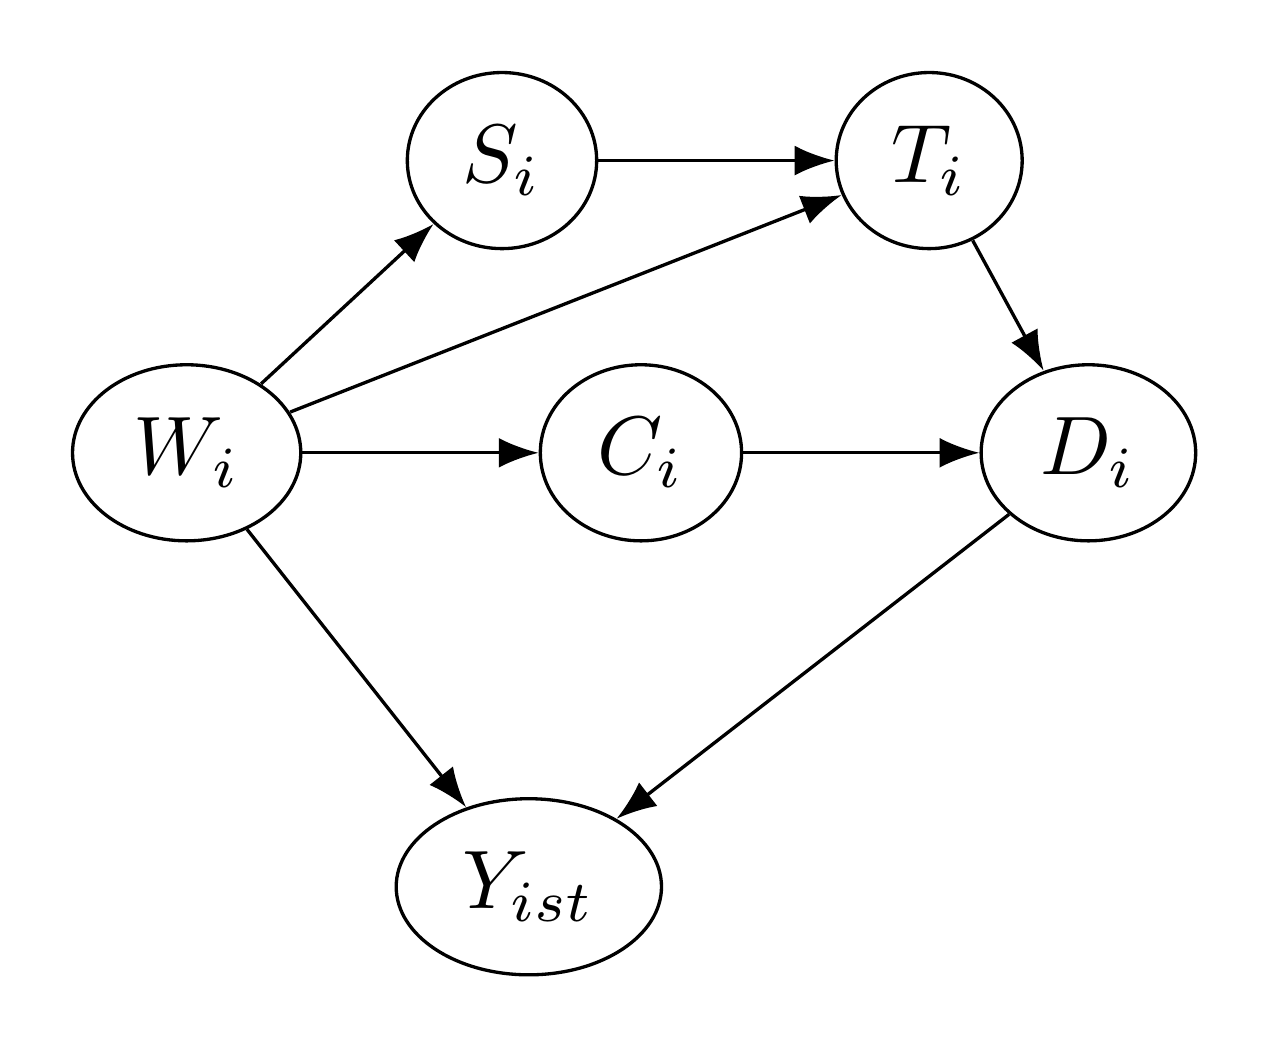
\includegraphics[width = 0.6\textwidth]{DAG2.png}
		\caption{Causal diagram indicating the conditional independence assumptions needed to estimate the PATT-C.\label{fig:DAG}}
		%\caption{\label{fig:DAG} here}
	\end{center}
\end{figure}

Interference undermines the framework because it creates more than two potential outcomes per participant, depending on the treatment receipt of other participants \citep{rubin1990}. We therefore assume no interference between units: 

\vskip 0.2in
\begin{assumption}{5}{}\label{sutva}
	The potential outcomes $Y_{isd}$ do not depend on $D_j$, $\forall j\neq i$. 
	%\begin{equation*}
	%Y_{isd}^{L_i} = Y_{isd}^{L_j},  \forall i \neq j
	
	%\end{equation*}
	%where $L_j$ is the treatment and sample assignment vector for unit $j$. 
\end{assumption} 

We additionally include Assumptions \ref{monotonicity} and \ref{ER}, which are made by \citet{Angrist1996} to ensure identifiability. The former assumption ensures that crossover is only possible from treatment to control:

\vskip 0.2in
\begin{assumption}{6}{}\label{monotonicity}
No defiers: 
\begin{equation*}
T_i \geq D_i, \qquad \forall \, i \, , \, d, t=\{0,1\}.
\end{equation*}
\end{assumption}
\noindent
Assumption \ref{ER} ensures treatment assignment affects the response only through the treatment received. In particular, the treatment effect may only be nonzero for compliers.

\begin{assumption}{7}{}\label{ER}
Exclusion restriction: For noncompliers,
\begin{equation*}
Y_{i11} = Y_{i10}, \qquad \forall \, i.
\end{equation*}  
\end{assumption}

\subsection{PATT-C}
The estimand of interest is the Population Average Treatment Effect on Treated Compliers (PATT-C):
%
\begin{equation}\label{tpatt}
\tau_{\text{PATT-C}} = \ex\left( Y_{i01} - Y_{i00} \mid S_i=0, D_i=1\right).
\end{equation}
%
PATT-C is interpreted as the complier-average causal effect estimated on the RCT sample extrapolated to what we would have observed in the population if treatment received $D_i$ is the same. The following theorem relates the treatment effect in the RCT to the treatment effect in the population. 

\vskip 0.2in
\begin{theorem}\label{thm1}
Under Assumptions \ref{consistency} -- \ref{ER},
\begin{equation}\label{tpatt-est}
\tau_{\text{PATT-C}} = \ex_{01}\left[  \ex\left(Y_{i11} \mid S_i=1, D_i=1, W_i\right)\right]
-\ex_{01}\left[  \ex\left(Y_{i10} \mid S_i=1, T_i =0, C_i =1, W_i\right) \right] 
\end{equation}

where $\ex_{01}\left[\ex(\cdot \mid\dots, W_i)\right]$ denotes the expectation with respect to the distribution of $W_i$ for population members who receive treatment.
\end{theorem}

\begin{proof}
We separate the expectation linearly into two terms and consider each individually.
\begin{align*}
\ex\left(Y_{i01} \mid S_i=0,D_i=1\right) &= \ex\left(Y_{i11} \mid S_i=0, D_i=1\right) \tag*{by Assumption \ref{consistency}} \\
&= \ex\left(Y_{i11} \mid S_i=0, T_i=1, C_i=1\right) \tag*{by Assumption \ref{monotonicity}} \\
&= \ex_{01}\left[  \ex\left(Y_{i11} \mid S_i=0, T_i=1, C_i=1, W_i\right) \right] \\
&= \ex_{01}\left[  \ex\left(Y_{i11} \mid S_i=1, T_i=1, C_i=1, W_i\right) \right] \tag*{by Assumption \ref{si_treat}} \\
&= \ex_{01}\left[  \ex\left(Y_{i11} \mid S_i=1, D_i=1, W_i\right)\right] 
\end{align*}

Intuitively, conditioning on $W_i$ makes sample selection ignorable under Assumption \ref{si_treat}. This is the critical connector between the third and fourth lines of the first expectation derivation.
	
\begin{align*}
\ex\left(Y_{i00} \mid S_i=0, D_i=1\right) &= \ex\left(Y_{i10} \mid S_i=0, D_i=1\right) \tag*{by Assumption \ref{consistency}} \\
&= \ex\left(Y_{i10} \mid S_i=0, T_i=1, C_i=1\right) \tag*{by Assumption \ref{monotonicity}} \\
&= \ex_{01}\left[  \ex\left(Y_{i10} \mid S_i=1, T_i=1, C_i=1, W_i\right) \right] \tag*{by Assumption \ref{si_ctrl}} \\
&= \ex_{01}\left[  \ex\left(Y_{i10} \mid S_i=1, T_i=0, C_i=1, W_i\right) \right] \tag*{by Assumption \ref{compl}}\\
\end{align*}

The last line follows because Assumption \ref{compl} allows us to use RCT controls who would have complied had they been assigned to treatment. Finally, the result follows by plugging these two expressions into Eq.~\eqref{tpatt}.
\end{proof}

\section{Estimation procedure}\label{estimation}
There are two challenges in turning Theorem~\ref{thm1} into an estimator of $\tau_{\text{PATT-C}}$ in practice. First, we must estimate the inner expectation over potential outcomes of compliers in the RCT. In the empirical example, we use an ensemble of algorithms \citep{van2007} to estimate the response surface for compliers in the RCT, given their covariates. Thus, the first term in the expression for $\tau_{\text{PATT-C}}$ is estimated by the weighted average of points on the response surface, evaluated for each treated population member's potential outcome under treatment. The second term is estimated by the weighted average of points on the response surface, evaluated for each treated population member's potential outcome under control.

The second challenge is that we cannot observe which individuals are included in the estimation of the second term. In the RCT control group, $C_i$ is unobservable, as they always receive no treatment ($D_i=0$). We must estimate the second term of Eq.~\eqref{tpatt-est} by predicting who in the control group would be a complier had they been assigned to treatment. An alternative approach is to simply weight the PATT estimate by the population compliance rate in order to yield a population average effect of treatment on treated compliers. However, the compliance rate is likely to differ between the sample and population, as well as across subgroups. Explicitly modeling compliance allows us to decompose PATT-C estimates by subgroup according to covariates common to both RCT and observational datasets.

The procedure for estimating $\tau_{\text{PATT-C}}$ using Theorem~\ref{thm1} is as follows:
\begin{enumerate}[label=\textbf{S.\arabic*},ref=S.\arabic*]
\item Using the group assigned to treatment in the RCT $(S_i=1, T_i=1)$, train a model (or an ensemble of models) to predict the probability of compliance as a function of covariates $W_i$. \label{compliance-model}
\item Using the model from \ref{compliance-model}, predict who in the RCT assigned to control \textit{would have} complied to treatment had they been assigned to the treatment group.\footnote{We use a standard prediction threshold of 50\% in order classify compliers, $C_i=1$. Adjusting the prediction threshold upward would result in more accurate classifications, although we do not explore this approach.} \label{complier-predict}
\item For the observed compliers assigned to treatment and predicted compliers assigned to control, train a model to predict the response using $W_i$ and $D_i$, which gives $\ex(Y_{i1d} \mid S_i=1, D_i=d, W_i)$ for $d \in \{0,1\}$.\label{response-model}
\item For all individuals who received treatment in the population $(S_i=0, D_i=1)$, estimate their potential outcomes using the model from \ref{response-model}, which gives $Y_{i1d}$ for $d \in \{0,1\}$. The mean counterfactual $Y_{i11}$ minus the mean counterfactual $Y_{i10}$ is the estimate of $\tau_{\text{PATT-C}}$.\label{response-predict}
\end{enumerate}

Assumptions \ref{si_treat} and \ref{si_ctrl} are particularly important for estimating $\tau_{\text{PATT-C}}$: the success of the proposed estimator hinges on the assumption that the response surface is the same for compliers in the RCT and target population. If this does not hold, then the potential outcomes $Y_{i10}$ and $Y_{i11}$ for target population individuals cannot be estimated using the model from \ref{response-model}.\footnote{Section \ref{verifying} discusses whether the strong ignorability assumptions are plausible in the empirical application.}

\subsection{Modeling assumptions}  \label{modeling-assumptions}

In addition to the identification assumptions, we require additional modeling assumptions for the estimation procedure. First, we assume that the $W_i$ that determine sample selection also determine population treatment assignment and complier status. As pointed out in Section \ref{assumptions}, we also require that $W_i$ is complete because if any relevant elements of $W_i$ are not controlled, then there is a backdoor pathway from $T_i$ back to $W_i$ and into $Y_{isd}$. Lastly, we assume that the compliance model is accurate in predicting compliance in the training sample of RCT participants assigned to treatment and also generalizable to RCT participants assigned to control (\ref{compliance-model} and \ref{complier-predict}). Section \ref{ensemble} below describes the method of evaluating the generalizability of the compliance model.

\subsection{Ensemble method}  \label{ensemble}

In the empirical application, we use the weighted ensemble method described in \citet{van2007} for \ref{compliance-model} and \ref{response-model} of the estimation procedure. This ensemble method combines algorithms with a convex combination of weights based on minimizing cross-validated error. It is shown to control for overfitting and outperforms single algorithms selected by cross-validation \citep{polley2010super}. 

We choose a variety of candidate algorithms to construct the ensemble, with a preference towards algorithms that tend to outperform in supervised classification tasks. We also have a preference for algorithms that have a built-in variable selection property. The idea is that we input the same $W_i$ and each candidate algorithm selects the most important covariates for predicting compliance status or potential outcomes.\footnote{A potential concern when predicting potential outcomes is that the algorithm might shrink the treatment received predictor to zero, which would result in no difference between counterfactual potential outcomes.} We select three types of candidate algorithms: nonparametric additive regression models \citep{buja1989linear}; L1 or L2-regularized linear models (i.e., Lasso or ridge regression, respectively) \citep{tibshirani2012strong}; and ensembles of decision trees (i.e., random forests) \citep{breiman2001}. L1-regularized linear models are important for the application due to their variable selection properties: Lasso is particularly attractive because it tends to shrink all but one of the coefficients of correlated covariates to zero. 

\section{Simulations} \label{sim}
We conduct a simulation study to compare the performance of the PATT and PATT-C estimators. For comparison, we compare the population estimates to the \textcolor{red}{sample Complier Average Causal Effect (CACE), which is the sample analog to PATT-C:
%
\begin{equation}\label{tcace}
\tau_{\text{CACE}} = \ex\left( Y_{i11} - Y_{i10} \mid S_i=1, C_i=1\right).
\end{equation}
%
The PATT and PATT-C estimates are obtained by estimating the response surface on all individuals in the RCT and applying \ref{response-predict} of the estimation procedure to the population members. Note that the PATT estimator described here is the population-average causal effect of taking up treatment, adjusted according to the covariate distribution of population ``compliers.'' In contrast, the \citet{Hartman} population estimator is the ITT estimator reweighted according the to covariate distribution of the population.}

\subsection{Simulation design}

The simulation is designed so that the effect of treatment is heterogeneous and depends on covariates which are different in the RCT and target population. The design satisfies the conditional independence assumptions in Figure~\ref{fig:DAG}.

In the simulation, RCT eligibility, complier status, and treatment assignment in the population depend on multivariate normal covariates $(W^{1}_i, W^{2}_i, W^{3}_i, W^{4}_i)$ with mean $(0.5, 1, -1, -1)$ and covariances $\cov(W^{1}_i, W^{2}_i) = \cov(W^{1}_i, W^{4}_i)= \cov(W^{2}_i, W^{4}_i) = \cov(W^{3}_i, W^{4}_i) = 1$ and $\cov(W^{1}_i, W^{3}_i) = \cov(W^{2}_i, W^{3}_i) = 0.5$.  The first three covariates are observed by the researcher and $W^{4}_i$ is unobserved. 

The  equation for selection into the RCT is
 \vskip 0.2in
 $$ S_i = \ind(e_2 + g_1W^{1}_i + g_2W^{2}_i + g_3W^{3}_i + e_4W^{4}_i + R > 0),$$
 \vskip 0.2in
\noindent
where $R$ is standard normal. The parameter $e_2$ varies the fraction of the population eligible for the RCT and $e_4$ varies the degree of confounding with sample selection. We set the constants $g_1, g_2,$ and $g_3$ to be $0.5,$ $0.25,$ and $0.75$, respectively.

Complier status is determined by
\vskip 0.2in
$$C_i = \ind(e_3 + h_2W^{2}_i + h_3W^{3}_i + e_5W^{4}_i + Q > 0),$$
\vskip 0.2in
\noindent
where $Q$ is standard normal, $e_3$ varies the fraction of compliers in the population, and $e_5$ varies the degree of confounding with treatment assignment. We set the constants $h_2$ and $h_3$ to $0.5$.

For individuals in the population ($S_i=0$), treatment is assigned by
 \vskip 0.2in
  $$T_i = \ind(e_1 + f_1W^{1}_i + f_2W^{2}_i + e_6W^{4}_i + V > 0),$$
  \vskip 0.2in
\noindent
where $V$ is standard normal. Varying $e_1$ changes the fraction eligible for treatment in the population and $e_6$ varies the degree of confounding with sample selection. We set the constants $f_1$ and $f_2$ to $0.25$ and $0.75$, respectively. For individuals in the RCT ($S_1=1$), treatment assignment is a sample from a Bernoulli distribution with probability $p=0.5$.
We set treatment received $D_i$ according to $T_i$ and $C_i$: $D_i = T_i$ if $C_i=1$ and $D_i = 0$ if $C_i=0$.

Finally, the response is determined by 
\vskip 0.2in
$$Y_{isd} = a + bD + c_1W^{1}_i + c_2W^{2}_i + dU.$$
\vskip 0.2in
We assume that the treatment effect $b$ is heterogeneous depending on $W^{1}_i$: $b = 1$ if $W^{1}_i > 0.75$ and $b=-1$ if $W^{1}_i \leq 0.75$.  We set $a, c_1,$ and $d$ to $1$ and $c_2$ to $2$. $U$ is standard normal and $U, V, R, Q, (W^{1}_i, W^{2}_i, W^{3}_i, W^{4}_i)$ are mutually independent.
 
We generate a population of 30,000 individuals and randomly sample 5,000. Those among the 5,000 who are eligible for the RCT ($S_i=1$) are selected. Similarly, we sample 5,000 individuals from the population and select those who are not eligible for the RCT ($S_i=0$): these are the observational study participants.\footnote{This set-up mimics the reality that a population census is usually impossible.}

We set each individual's treatment received $D_i$ according to their treatment assignment and complier status and observe their responses $Y_{isd}$. In this design, the manner in which $S_i$, $T_i$, $D_i$, $C_i$, and $Y_{isd}$ are simulated ensures that Assumptions \ref{consistency} -- \ref{ER} hold.

In the assigned-treatment RCT group $(S_i = 1, T_i = 1)$, we train a gradient boosting algorithm \citep{friedman2001greedy} on the covariates to predict who in the control group $(S_i = 1, T_i = 0)$ would comply with treatment ($C_i=1$), which is unobservable. These individuals \textit{would have} complied had they been assigned to the treatment group. For this group of observed compliers to treatment and predicted compliers from the control group of the RCT, we estimate the response surface using gradient boosting with features $(W^{1}_i, W^{2}_i, W^{3}_i)$ and $D_i$. The PATT-C is estimated according to the estimation procedure outlined above.

\subsection{Simulation results}\label{sim-results}

We vary each of the parameters $e_1, e_2$, $e_3$, $e_4$, $e_5$, and $e_6$ along a grid of five random standard normal values in order to generate different combinations of rates of compliance, treatment eligibility, RCT eligibility in the population, and confounding. For each possible combination of the six parameters, we run the simulation ten times and compute the average root mean squared error (RMSE) of PATT-C, PATT, and the CACE. All other parameters are held constant. 

Figure~\ref{fig:rmse_ratec_rates} shows the relationship between the percent of compliers in the whole population, the percentage of people in the population eligible to participate in the RCT, and the RMSE of the PATT and PATT-C estimators. The PATT estimator performs badly when the compliance rate is low, whereas the PATT-C estimator is comparatively insensitive to changes in the compliance rate. A similar pattern emerges when the compliance rate varies with the population treatment rate (Figure~\ref{fig:rmse_ratec_ratet}).

\begin{figure}[htbp]
	\begin{center}
		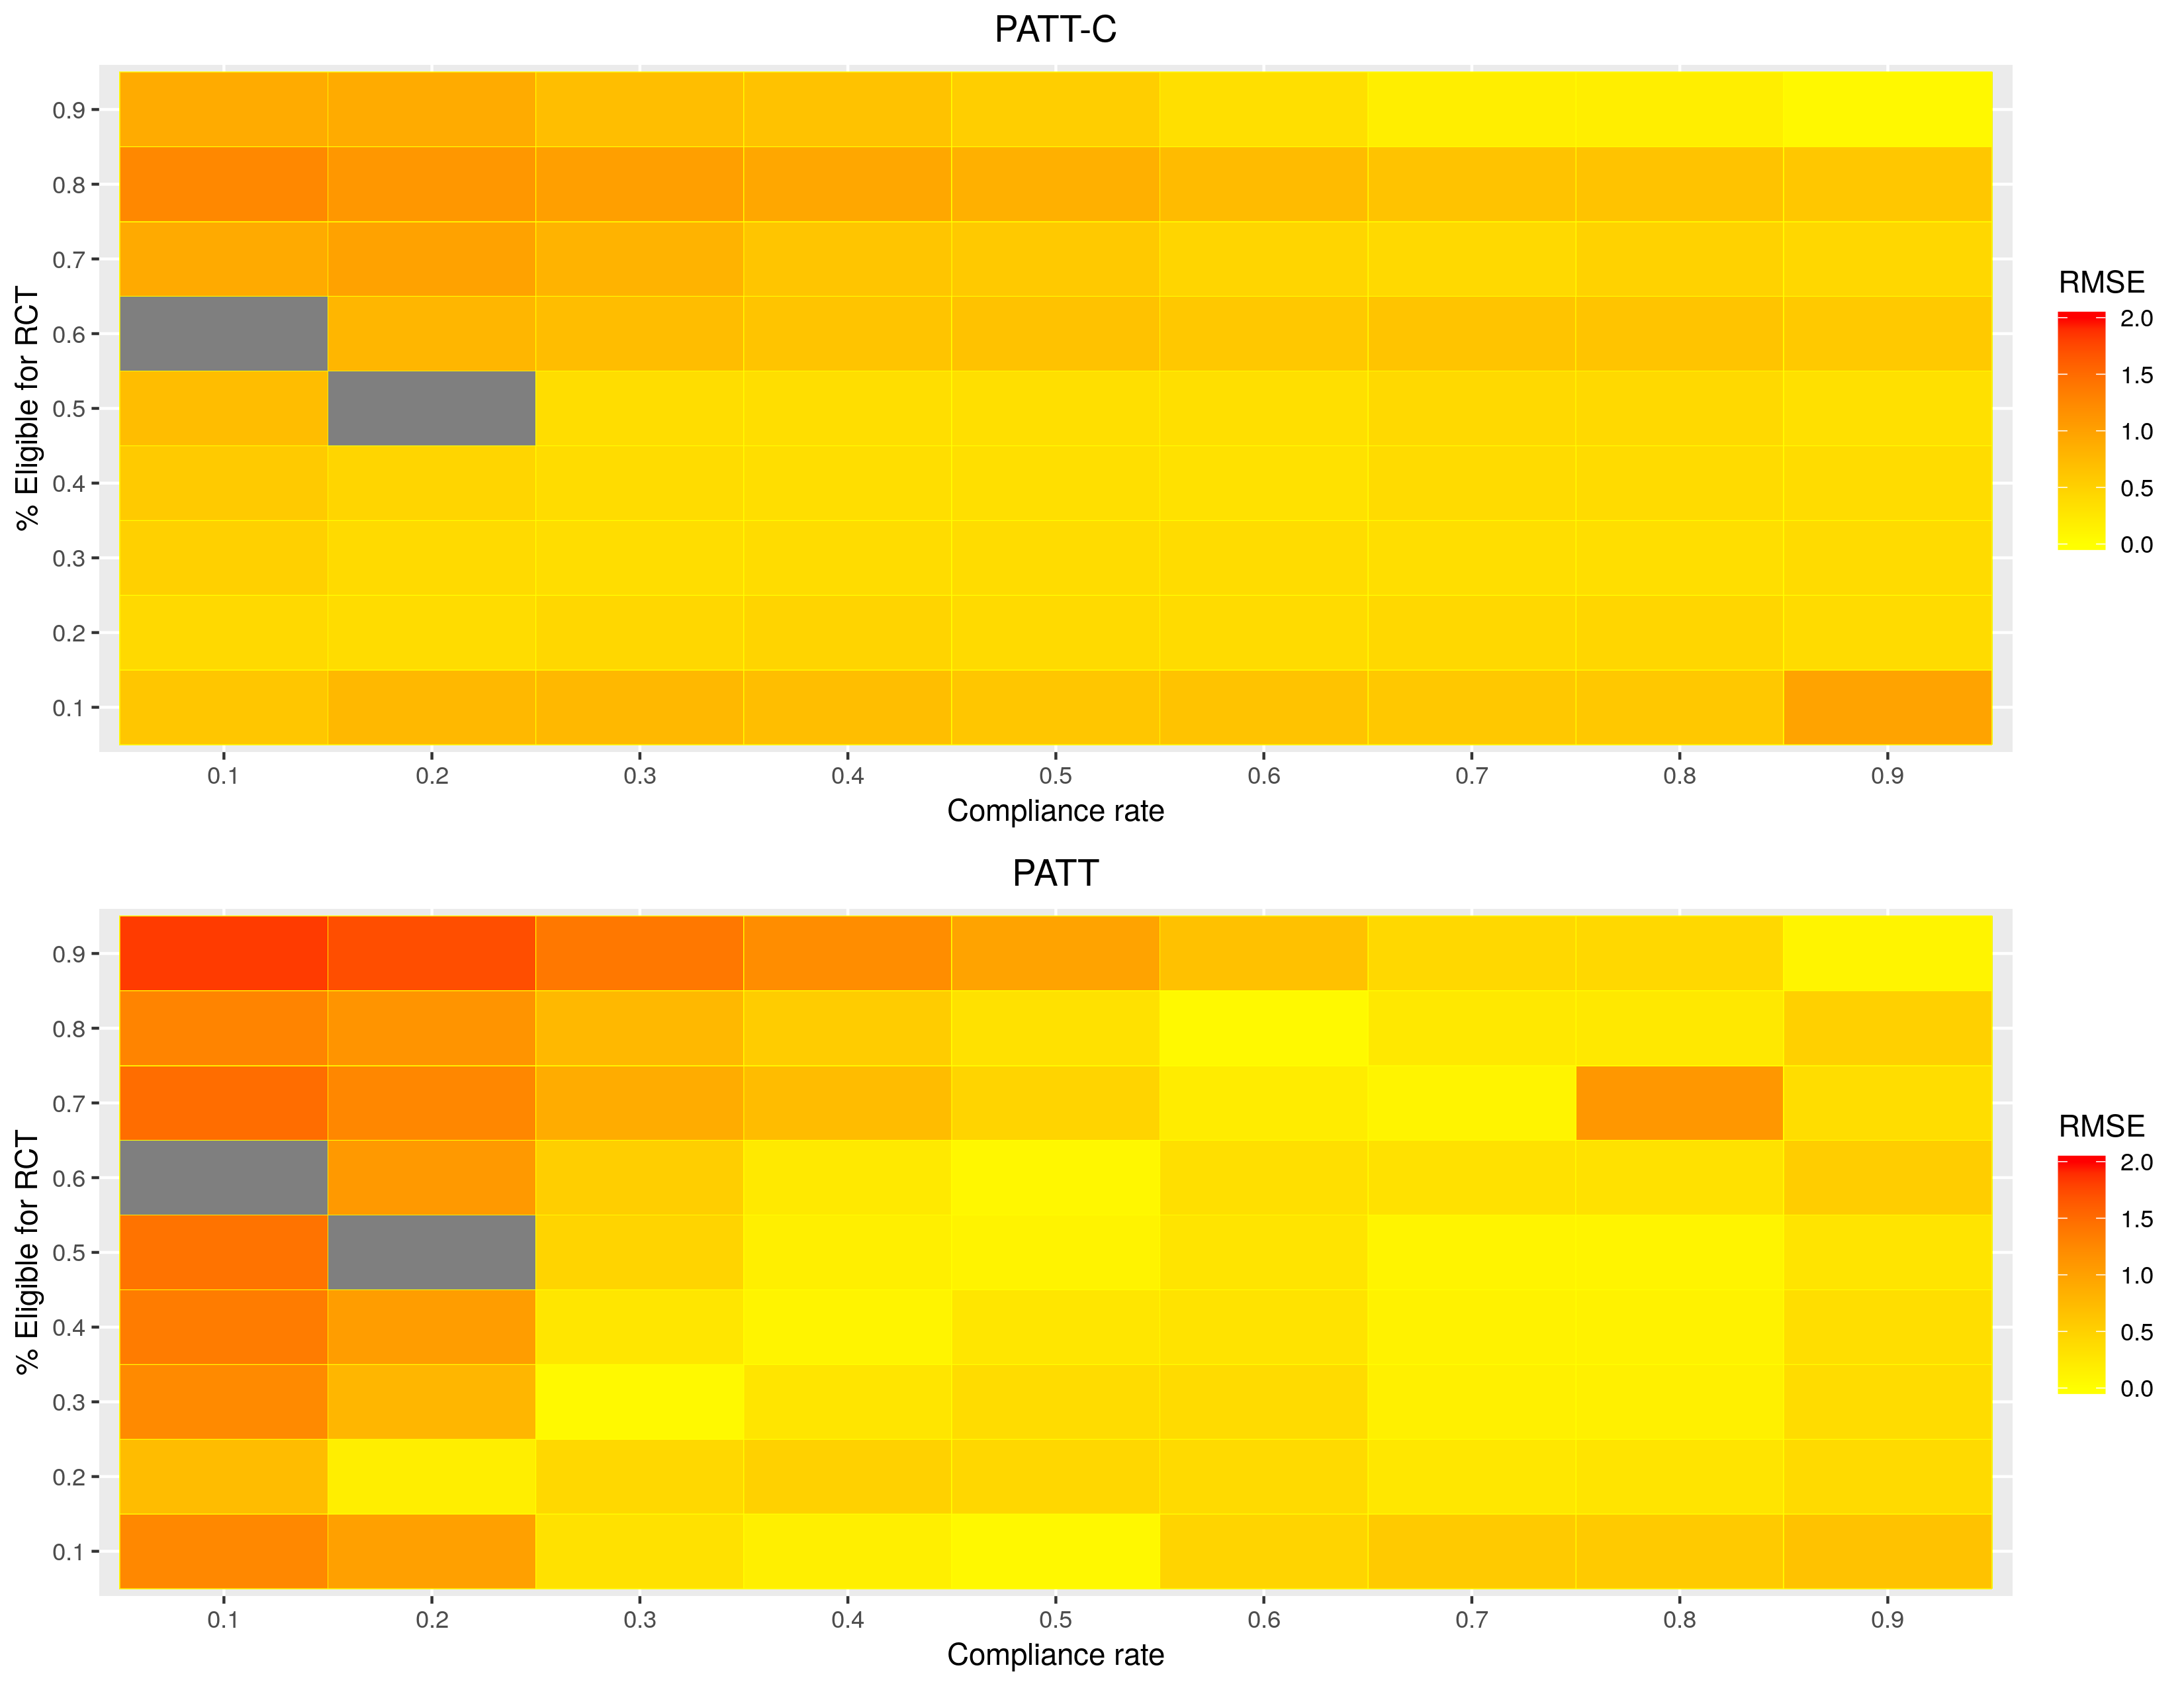
\includegraphics[width = 1\textwidth]{rmse_ratec_rates.png}
		\caption{Simulated RMSE, binned by compliance rate and percent eligible for the RCT. Darker tiles correspond to higher errors and white tiles correspond to missing simulated data.\label{fig:rmse_ratec_rates}}
%		\caption{\label{fig:rmse_ratec_rates} here}
	\end{center}
\end{figure}

Figure~\ref{fig:rmse_boxplots_rateC} compares the RMSE of PATT and PATT-C with the CACE at varying levels of compliance in the total population. PATT-C is relatively invariant to changes in the compliance rate and outperforms both PATT and CACE in terms of minimizing RMSE when the compliance rate is below 70\%. For high levels of compliance, the CACE \textcolor{red}{performs comparably to the PATT or PATT-C estimators}.  

Figures~\ref{fig:rmse_boxplots_RateConC}, \ref{fig:rmse_boxplots_RateConT}, and \ref{fig:rmse_boxplots_RateConS} explore how the degrees of confounding in the mechanisms that determine sample selection, treatment assignment, and compliance affect estimation error. PATT-C tends to be invariant to increases in the degree of confounding, whereas PATT is sensitive to confounding in the sample selection mechanism. The CACE estimates are generally more variable than the population estimates due to the sample estimator's inability to account for differences in pretreatment covariates between the RCT sample and target population. 

\begin{figure}[htbp]
\begin{center}
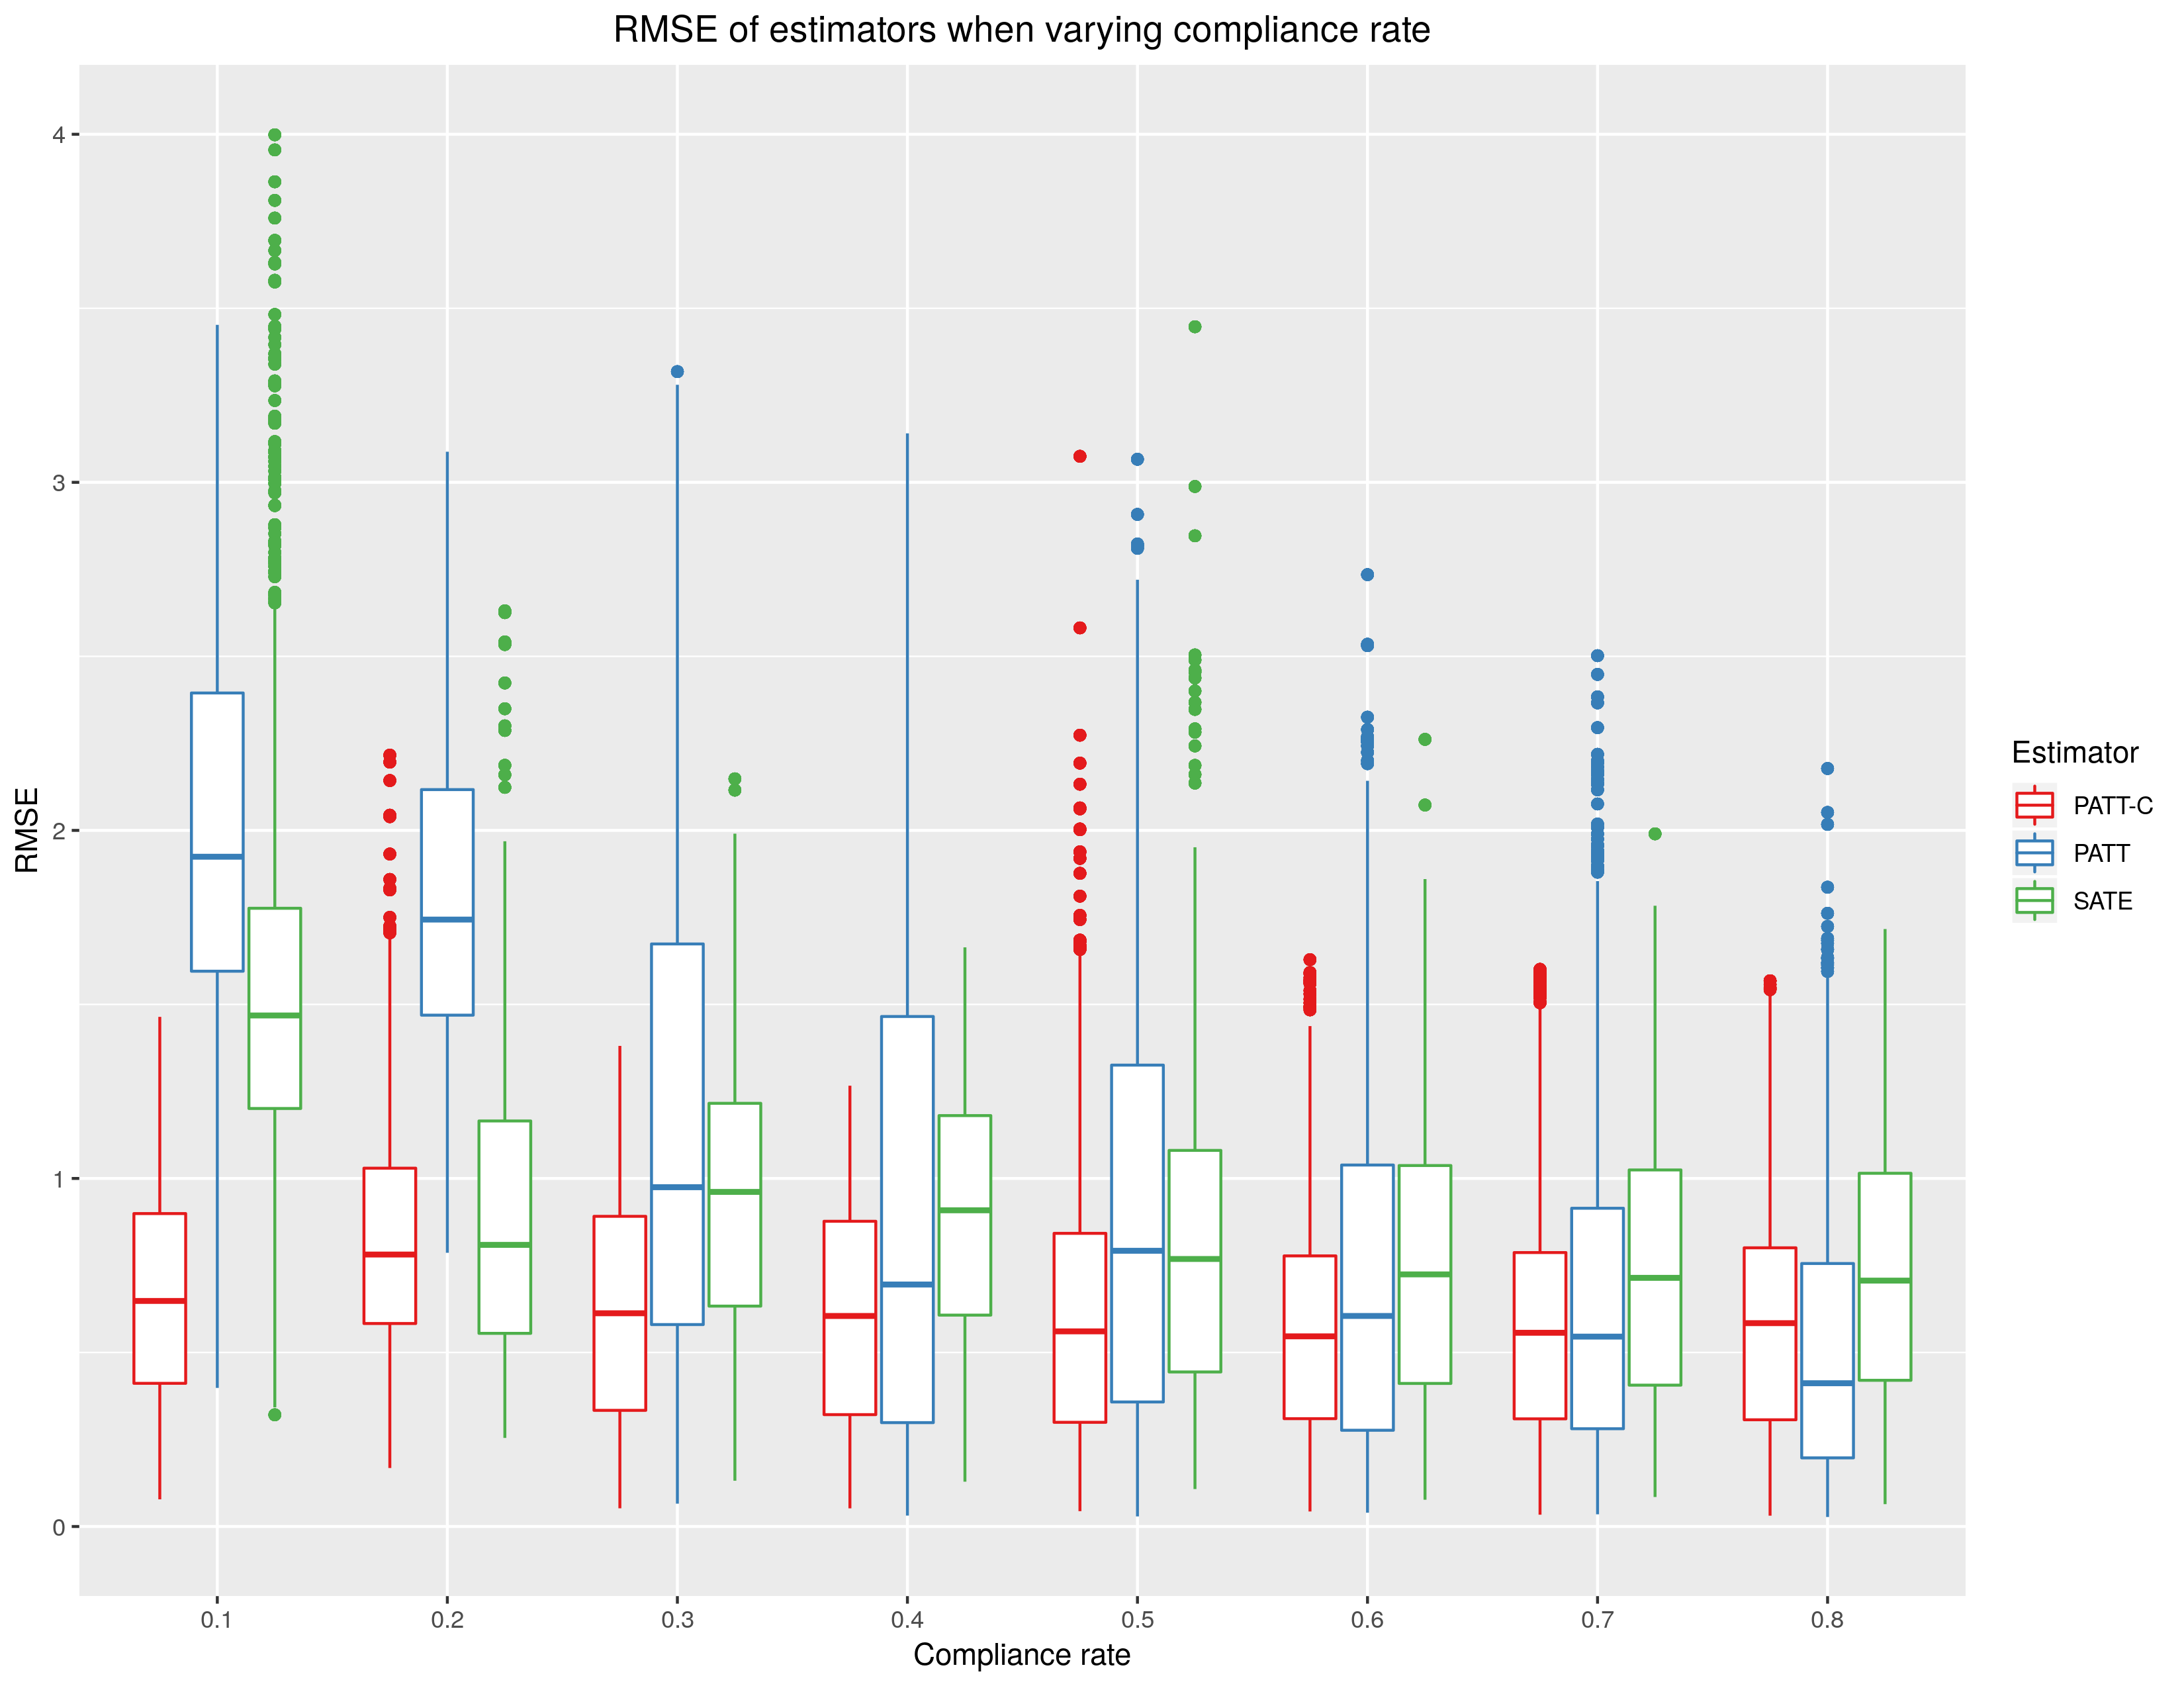
\includegraphics[width = 1\textwidth]{rmse_boxplots_rateC.png}
\caption{Simulated RMSE of PATT-C, PATT, and CACE, according to compliance rates in the total population.\label{fig:rmse_boxplots_rateC}}
%\caption{\label{fig:rmse_boxplots_rateC} here}
\end{center}
\end{figure}

\pagebreak
\section{Application: Medicaid and health care use} \label{application}

We apply the proposed estimator to measure the effect of Medicaid coverage on health care use for a target population of adults who may benefit from expansions to the Medicaid program. In particular, we examine the population of nonelderly adults in the U.S. with household incomes at or below 138\% of the Federal Poverty Level (FPL) --- which amounts to \$32,913 for a four--person household in 2014 --- who may be eligible for Medicaid following the Affordable Care Act (ACA) expansion.

\subsection{RCT sample} 

We draw RCT data from the Oregon Health Insurance Experiment (OHIE) \citep{finkelstein2012,baicker2013,baicker2014,Taubman}. In 2008, approximately 90,000 uninsured low-income adults participated in the OHIE to receive Medicaid benefits.\footnote{Eligible participants include Oregon residents (US citizens or legal immigrants) aged 19 to 64 not otherwise eligible for public insurance, who have been without insurance for six months, and have income below the FPL and assets below \$2,000.} Treatment occurred at the household level: participants selected by the lottery won the opportunity for themselves and any household member to apply for Medicaid. Within a sample of 74,922 individuals representing 66,385 households, 29,834 participants were selected by the lottery; the remaining 45,008 participants served as controls in the experiment. Participants in selected households received benefits if they returned an enrollment application within 45 days of receipt. Among participants in selected households, about 60\% mailed back applications and only 30\% successfully enrolled.\footnote{About half of the returned applications were deemed ineligible, primarily due to failure to demonstrate income below the FPL. Enrolled participants were required to recertify their eligibility status every six months.}

The response data originate from a mail survey that was administered to participants over July and August 2009 ($n = 23,741$ survey respondents). We use the same definition of insurance coverage as \citet{finkelstein2012} to form the measure of compliance, which is a binary variable indicating whether the participant was enrolled in any Medicaid program during the study period. The OHIE data include pretreatment covariates for gender, age, race, ethnicity, health status, education, and household income.  

The outcomes of interest are binary variables for any emergency room (ER) and outpatient visits in the past 12 months. ER use is an important outcome because it is the main delivery system through which the the uninsured receive health care. The uninsured could potentially receive higher quality and less affordable health care through outpatient visits. An important question for policymakers is whether Medicaid expansions will decrease ER utilization by the previously uninsured.   	

Subsequent research calls in to question the external validity of the OHIE, which resulted in the counterintuitive finding that Medicaid increased ER use among RCT participants \citep{finkelstein2012,Taubman}. For example, quasi-experimental studies on the impact of the 2006 Massachusetts health reform --- which served as a model for the ACA --- show that ER use decreased or remained constant following the reform \citep{miller2012effect, kolstad2012impact}. A challenge to the external validity of the OHIE is that it's exclusion criteria was likely more restrictive than government health insurance expansions. 

\subsection{Observational data} 

We acquire data on the target population from the National Health Interview Study (NHIS) for years 2008 to 2017.\footnote{A possible limitation of this application is that it ignores the complex sampling techniques of the NHIS sample design such as differential sampling, which is discussed in detail in \citet{parsons2014design}.} We restrict the sample to respondents with income below 138\% of the FPL and who are uninsured or on Medicaid and select covariates on respondent characteristics that match the OHIE pretreatment covariates. The outcomes of interest from NHIS are variables on ER and outpatient visits in the past 12 months. We use a recoded variable that indicates whether respondents are on Medicaid as an analogue to the OHIE compliance measure. 

\subsection{Verifying assumptions} \label{verifying}

In order for $\tau_{\text{PATT-C}}$ to be identified, Assumptions \ref{consistency} -- \ref{ER} must be met. Assumption \ref{consistency} ensures that potential outcomes for participants in the target population would be identical to their outcomes in the RCT if they had been randomly assigned their observed treatment. In the empirical application, Medicaid coverage for uninsured individuals was applied in the same manner in the RCT as it is in the population.  Differences in potential outcomes due to sample selection might arise, however, if there are differences in the mail surveys used to elicit health care use responses between the RCT and the nonrandomized study. 

We cannot directly test Assumptions \ref{si_treat} and \ref{si_ctrl}, which state that potential outcomes for treatment and control are independent of sample assignment for individuals with the same covariates and assignment to treatment. The assumptions are only met if every possible confounder associated with the response and the sample assignment is accounted for. In estimating the response surface, we use all demographic, socioeconomic, and pre-existing health condition data that were common in the OHIE and NHIS data. Potentially important unobserved confounders include the number of hospital and outpatient visits in the previous year, proximity to health services, and enrollment in other federal programs. 

The final two columns of Table~\ref{rct-nrt-compare} compares RCT participants selected for Medicaid with population members on Medicaid. Compared to the RCT compliers, the target population ``compliers''  are predominantly female, younger, more racially and ethnically diverse, less educated, and live in higher income households. Diagnoses of diabetes, asthma, high blood pressure, and heart disease are more common among the population on Medicaid then the RCT treated.

Strong ignorability assumptions may also be violated due to the fact that the OHIE applied a more stringent exclusion criteria compared to the NHIS sample. While the RCT and population sample both screened for individuals below the FPL, only the RCT required those enrolled to recertify their eligibility status every six months.

A violation of no-interference (Assumption \ref{sutva}) biases the estimate of $\tau_{\text{PATT-C}}$ if, for instance, treated participants' Medicaid coverage makes control participants more likely to visit the ER. Interference is less likely in this experimental set--up because treatment occurs at the household level. 

Assumption \ref{compl} is violated if assignment to treatment influences the compliance status of individuals with the same covariates. The compliance ensemble can accurately classify compliance status for 77\% of treated RCT participants with only the covariates --- and not treatment assignment --- as model inputs.\footnote{The compliance ensemble is evaluated in terms of 10--fold cross--validated MSE. The distribution of MSE for the ensemble and its candidate algorithms are provided in Table \ref{compliance-ensemble}.}  This gives evidence in favor of the conditional independence assumption.

The exclusion restriction (Assumption \ref{ER}) ensures treatment assignment affects the response only through enrollment in Medicaid. It is reasonable that a person's enrollment in Medicaid, not just their eligibility to enroll, would affect their hospital use. For private health insurance one might argue that eligibility may be be negatively correlated with hospital use, as people with pre-existing conditions are less often eligible yet go to the hospital more frequently. This should not be the case with a federally funded program such as Medicaid. 

\subsubsection{Placebo tests} \label{placebo-tests}

Similar to the procedure proposed by \citep{Hartman}, we conduct placebo tests to check whether the average outcomes differ between the RCT compliers on Medicaid and the adjusted population ``compliers'' on Medicaid.\footnote{Note that a placebo test for Assumption \ref{compl} is not possible because we never observe whether RCT controls would actually take-up treatment if assigned.} If the placebo tests detect a significant difference between the mean outcomes of these groups, it would indicate that either Assumption \ref{consistency} (for $d=1$), or Assumptions \ref{si_treat} and \ref{si_ctrl} are violated. 

Table \ref{placebo} reports the results of placebo tests, comparing the mean outcomes of RCT compliers against the mean outcomes of adjusted population ``compliers." The former quantity is calculated from the observed RCT sample and the latter quantity is the mean counterfactual $Y_{i11}$ estimated from \ref{response-predict} of the estimation procedure. Tests of equivalence between the two groups indicate that the differences across each outcome are not statistically significant. These results imply that the PATT-C estimator is not biased by differences in how Medicaid is delivered or health outcomes are measured between the RCT and population, or by differences in sample or population members' unobserved characteristics. 

\subsubsection{Sensitivity to no defiers assumption} \label{sens-defiers}

\citet{Angrist1996} show that the bias due to violations of Assumption \ref{monotonicity} is equivalent to the difference of average causal effects of treatment received for compliers and defiers, multiplied by the relative proportion of defiers, 
$\pr(i\text{ is a defier}) / (\pr(i\text{ is a complier]}) - \pr(i\text{ is a defier})).$

Table \ref{ohie-status} reports the distribution of participants in the OHIE by status of treatment assignment and treatment received. Assumption \ref{monotonicity} does not hold due to the presence of defiers; i.e., participants who were assigned to control and enrolled in Medicaid during the study period. About 6.7\% of the RCT sample were assigned to control but were enrolled in Medicaid ($T_i < D_i$) and 65.5\% of the sample complied with treatment assignment ($D_i = T_i$), which results in a bias multiplier of 0.11. Suppose that the difference of average causal effects of Medicaid received on ER use for compliers and defiers is 1.2\%. The resulting bias is only 0.1\%, which would not meaningfully alter the interpretation of the CACE or PATT-C estimates reported below. 
 
\subsection{Empirical results}\label{results}

We compare PATT-C and PATT estimates for ER and outpatient use. We obtain estimates for the overall group of participants and subgroups according to sex, age, race, health status, education, and household income. Subgroup treatment effects are estimated by taking differences across response surfaces for a given covariate subgroup, and response surfaces are estimated with the ensemble mean predictions. We use treatment received, number of household members, and the subgroup covariates as features in the response models. We generate 95\% confidence intervals for these estimates using 1,000 bootstrap samples. 

Table \ref{compliance-compare} presents the PATT-C estimates, which indicate that Medicaid coverage has a positive, but considerably smaller effect on the number of ER and outpatient visits. For comparison, \citet{finkelstein2012} reports population estimates of the effect of Medicaid coverage on the number of ER and out-patient visits using 2004--2009 NHIS data on adults aged 19--64 below 100 percent of the federal poverty line ($n=15,528$). \citet{finkelstein2012} estimates Medicaid coverage significantly increases the number of ER visits by 0.08 [0.05, 0.12] and increases the number of outpatient visits by 1.45 [1.33, 1.57]. 

Figures \ref{fig:any-visit-plot}, \ref{fig:num-visit-plot}, and \ref{fig:num-out-plot} examine heterogeneous treatment effect estimates on ER and outpatient use in the population. While this study is the first to our knowledge to estimate heterogeniety in treatment effects for the target population, \citet{Taubman} and \citet{NBERw22363} perform subgroup analyses on the RCT sample. Similar to the PATT-C estimates, \possessivecite{Taubman} subgroup analyses indicate that increases in ER use due to Medicaid are significantly larger for younger individuals and those with high school-level education.\footnote{\citet{NBERw22363} perform subgroup analyses on OHIE sample data and find larger increases in ER use as a result of Medicaid for men, English speakers, and individuals enrolled in a food stamp program prior to the lottery.}

\section{Discussion} \label{discussion}

The simulation results presented in Section \ref{sim} show that the PATT-C estimator outperforms its unadjusted counterpart when the compliance rate is low. Of course, the simulation results depend on the particular way we parameterized the compliance, selection, treatment assignment, and response schedules. 

In particular, the strength of correlation between the covariates and compliance governs how well the estimator will perform, since \ref{compliance-model} of the estimation procedure is to predict who \textit{would be} a complier in the RCT control group, had they been assigned to treatment. If it is difficult to predict compliance using the observed covariates, then the estimator will perform badly because of noise introduced by incorrectly treating noncompliers as compliers. Further research should be done into ways to test how well the model of compliance works in the population or explore models to more accurately predict compliance in RCTs.  Accurately predicting compliance is not only essential for yielding unbiased estimates of the average causal effects for target populations, it is also useful for researchers and policymakers to know which groups of individuals are unlikely to comply with treatment. 

In the OHIE trial, only about $30\%$ of those selected to receive Medicaid benefits actually enrolled. The compliance ensemble accurately classified compliance status for 77\% of treated RCT participants using only the pretreatment covariates as features. While we don't know how well the compliance ensemble predicts for the control group, the control group should be similar to the treatment group on pretreatment covariates because of the RCT randomization. The model's performance on the training set suggests that compliance is not purely random and depends on observed covariates. This gives evidence in favor of using the proposed estimator. 

In the empirical application, the sample population differs in several dimensions from the target population of individuals who will be covered by other Medicaid expansions, such as the ACA expansion to cover all adults up to 138\% of the FPL. For instance, the RCT participants are disproportionately white urban--dwellers \citep{Taubman}. The RCT participants volunteered for the study and therefore may be in poorer health compared to the target population. These differences in baseline covariates make reweighting or response surface methods necessary to extend the RCT results to the population.

Explicitly modeling compliance allows us to decompose population estimates by subgroup according to pretreatment covariates common to both RCT and observational datasets; e.g, demographic variables, pre--existing conditions, and insurance coverage. We find substantial differences between sample and population estimates in terms of race, education, and health status subgroups. This pattern is expected because RCT participants volunteered for the study and are predominately white and educated.

\pagebreak

%Bibliography
%\printbibliography

%Bibliography
\bibliographystyle{chicago}
\begin{thebibliography}{}
	
	\bibitem[\protect\citeauthoryear{Angrist, Imbens, and Rubin}{Angrist
		et~al.}{1996}]{Angrist1996}
	Angrist, J.~D., G.~W. Imbens, and D.~B. Rubin (1996, June).
	\newblock Identification of causal effects using instrumental variables.
	\newblock {\em Journal of the American Statistical Association\/}~{\em
		91\/}(434), 444--455.
	
	\bibitem[\protect\citeauthoryear{Baicker, Finkelstein, Song, and
		Taubman}{Baicker et~al.}{2014}]{baicker2014}
	Baicker, K., A.~Finkelstein, J.~Song, and S.~Taubman (2014).
	\newblock The impact of Medicaid on labor market activity and program
	participation: Evidence from the Oregon health insurance experiment.
	\newblock {\em The American Economic Review\/}~{\em 104\/}(5), 322.
	
	\bibitem[\protect\citeauthoryear{Baicker, Taubman, Allen, Bernstein, Gruber,
		Newhouse, Schneider, Wright, Zaslavsky, and Finkelstein}{Baicker
		et~al.}{2013}]{baicker2013}
	Baicker, K., S.~L. Taubman, H.~L. Allen, M.~Bernstein, J.~H. Gruber, J.~P.
	Newhouse, E.~C. Schneider, B.~J. Wright, A.~M. Zaslavsky, and A.~N.
	Finkelstein (2013).
	\newblock The Oregon experiment --- effects of Medicaid on clinical outcomes.
	\newblock {\em New England Journal of Medicine\/}~{\em 368\/}(18), 1713--1722.
	
	\bibitem[\protect\citeauthoryear{Breiman}{Breiman}{2001}]{breiman2001}
	Breiman, L. (2001).
	\newblock Random forests.
	\newblock {\em Machine Learning\/}~{\em 45\/}(1), 5--32.
	
	\bibitem[\protect\citeauthoryear{Buja, Hastie, and Tibshirani}{Buja
		et~al.}{1989}]{buja1989linear}
	Buja, A., T.~Hastie, and R.~Tibshirani (1989).
	\newblock Linear smoothers and additive models.
	\newblock {\em The Annals of Statistics\/}, 453--510.
	
	\bibitem[\protect\citeauthoryear{Finkelstein, Taubman, Wright, Bernstein,
		Gruber, Newhouse, and Allen}{Finkelstein et~al.}{2012}]{finkelstein2012}
	Finkelstein, A., S.~Taubman, B.~Wright, M.~Bernstein, J.~Gruber, J.~P.
	Newhouse, and H.~Allen (2012).
	\newblock The Oregon health insurance experiment: Evidence from the first year.
	\newblock {\em The Quarterly Journal of Economics\/}~{\em 127\/}(3), 1057.
	
	\bibitem[\protect\citeauthoryear{Friedman}{Friedman}{2001}]{friedman2001greedy}
	Friedman, J.~H. (2001).
	\newblock Greedy function approximation: {A} gradient boosting machine.
	\newblock {\em Annals of Statistics\/}, 1189--1232.
	
	\bibitem[\protect\citeauthoryear{Hartman, Grieve, Ramsahai, and Sekhon}{Hartman
		et~al.}{2015}]{Hartman}
	Hartman, E., R.~Grieve, R.~Ramsahai, and J.~S. Sekhon (2015).
	\newblock From SATE to PATT: Combining experimental with observational studies
	to estimate population treatment effects.
	\newblock {\em Journal of the Royal Statistical Society: Series A (Statistics
		in Society)\/}~{\em 10}, 1111.
	
	\bibitem[\protect\citeauthoryear{Imai, King, and Stuart}{Imai
		et~al.}{2008}]{ImaKinStu08}
	Imai, K., G.~King, and E.~Stuart (2008).
	\newblock Misunderstandings among experimentalists and observationalists about
	causal inference.
	\newblock {\em Journal of the Royal Statistical Society, Series A\/}~{\em 171,
		part 2}, 481{\textendash}502.
	
	\bibitem[\protect\citeauthoryear{Imai, Tingley, and Yamamoto}{Imai
		et~al.}{2013}]{imai2013experimental}
	Imai, K., D.~Tingley, and T.~Yamamoto (2013).
	\newblock Experimental designs for identifying causal mechanisms.
	\newblock {\em Journal of the Royal Statistical Society: Series A (Statistics
		in Society)\/}~{\em 176\/}(1), 5--51.
	
	\bibitem[\protect\citeauthoryear{Kolstad and Kowalski}{Kolstad and
		Kowalski}{2012}]{kolstad2012impact}
	Kolstad, J.~T. and A.~E. Kowalski (2012).
	\newblock The impact of health care reform on hospital and preventive care:
	Evidence from {M}assachusetts.
	\newblock {\em Journal of Public Economics\/}~{\em 96\/}(11-12), 909--929.
	
	\bibitem[\protect\citeauthoryear{Kowalski}{Kowalski}{2016}]{NBERw22363}
	Kowalski, A.~E. (2016, June).
	\newblock Doing more when you're running {LATE}: Applying marginal treatment
	effect methods to examine treatment effect heterogeneity in experiments.
	\newblock Working Paper 22363, National Bureau of Economic Research.
	
	\bibitem[\protect\citeauthoryear{Miller}{Miller}{2012}]{miller2012effect}
	Miller, S. (2012).
	\newblock The effect of insurance on emergency room visits: an analysis of the
	2006 {M}assachusetts health reform.
	\newblock {\em Journal of Public Economics\/}~{\em 96\/}(11-12), 893--908.
	
	\bibitem[\protect\citeauthoryear{Parsons, Moriarity, Jonas, Moore, Davis, and
		Tompkins}{Parsons et~al.}{2014}]{parsons2014design}
	Parsons, V.~L., C.~L. Moriarity, K.~Jonas, T.~F. Moore, K.~E. Davis, and
	L.~Tompkins (2014).
	\newblock Design and estimation for the {N}ational {H}ealth {I}nterview
	{S}urvey, 2006--2015.
	\newblock {\em National Center for Health Statistics. Vital and Health
		Statistics\/}~{\em 2\/}(165), 1--53.
	
	\bibitem[\protect\citeauthoryear{Polley and Van Der~Laan}{Polley and Van
		Der~Laan}{2010}]{polley2010super}
	Polley, E.~C. and M.~J. Van Der~Laan (2010).
	\newblock Super learner in prediction.
	\newblock Working Paper 266, Division of Biostatistics, University of
	California, Berkeley.
	
	\bibitem[\protect\citeauthoryear{Rubin}{Rubin}{1990}]{rubin1990}
	Rubin, D.~B. (1990).
	\newblock Comment: Neyman (1923) and causal inference in experiments and
	observational studies.
	\newblock {\em Statistical Science\/}~{\em 5\/}(4), 472--480.
	
	\bibitem[\protect\citeauthoryear{Stuart, Cole, Bradshaw, and Leaf}{Stuart
		et~al.}{2011}]{stuart2011use}
	Stuart, E.~A., S.~R. Cole, C.~P. Bradshaw, and P.~J. Leaf (2011).
	\newblock The use of propensity scores to assess the generalizability of
	results from randomized trials.
	\newblock {\em Journal of the Royal Statistical Society: Series A (Statistics
		in Society)\/}~{\em 174\/}(2), 369--386.
	
	\bibitem[\protect\citeauthoryear{Taubman, Allen, Wright, Baicker, and
		Finkelstein}{Taubman et~al.}{2014}]{Taubman}
	Taubman, S., H.~Allen, B.~Wright, K.~Baicker, and A.~Finkelstein (2014,
	January).
	\newblock Medicaid increases emergency department use: Evidence from Oregon's
	health insurance experiment.
	\newblock {\em Science\/}~{\em 343\/}(6168), 263--268.
	
	\bibitem[\protect\citeauthoryear{Tibshirani, Bien, Friedman, Hastie, Simon,
		Taylor, and Tibshirani}{Tibshirani et~al.}{2012}]{tibshirani2012strong}
	Tibshirani, R., J.~Bien, J.~Friedman, T.~Hastie, N.~Simon, J.~Taylor, and R.~J.
	Tibshirani (2012).
	\newblock Strong rules for discarding predictors in lasso-type problems.
	\newblock {\em Journal of the Royal Statistical Society: Series B (Statistical
		Methodology)\/}~{\em 74\/}(2), 245--266.
	
	\bibitem[\protect\citeauthoryear{van~der Laan, Polley, and Hubbard}{van~der
		Laan et~al.}{2007}]{van2007}
	van~der Laan, M.~J., E.~C. Polley, and A.~E. Hubbard (2007).
	\newblock Super learner.
	\newblock {\em Statistical Applications in Genetics and Molecular
		Biology\/}~{\em 6\/}(1).
	
\end{thebibliography}

%Appendix
\pagebreak
\begin{appendices}
	
% Appendix numbering
\newcommand{\hbAppendixPrefix}{A}
%
\renewcommand{\thefigure}{\hbAppendixPrefix\arabic{figure}}
\setcounter{figure}{0}
\renewcommand{\thetable}{\hbAppendixPrefix\arabic{table}} 
\setcounter{table}{0}
\renewcommand{\theequation}{\hbAppendixPrefix\arabic{equation}} 
\setcounter{equation}{0}


\begin{figure}[htbp]
	\begin{center}
		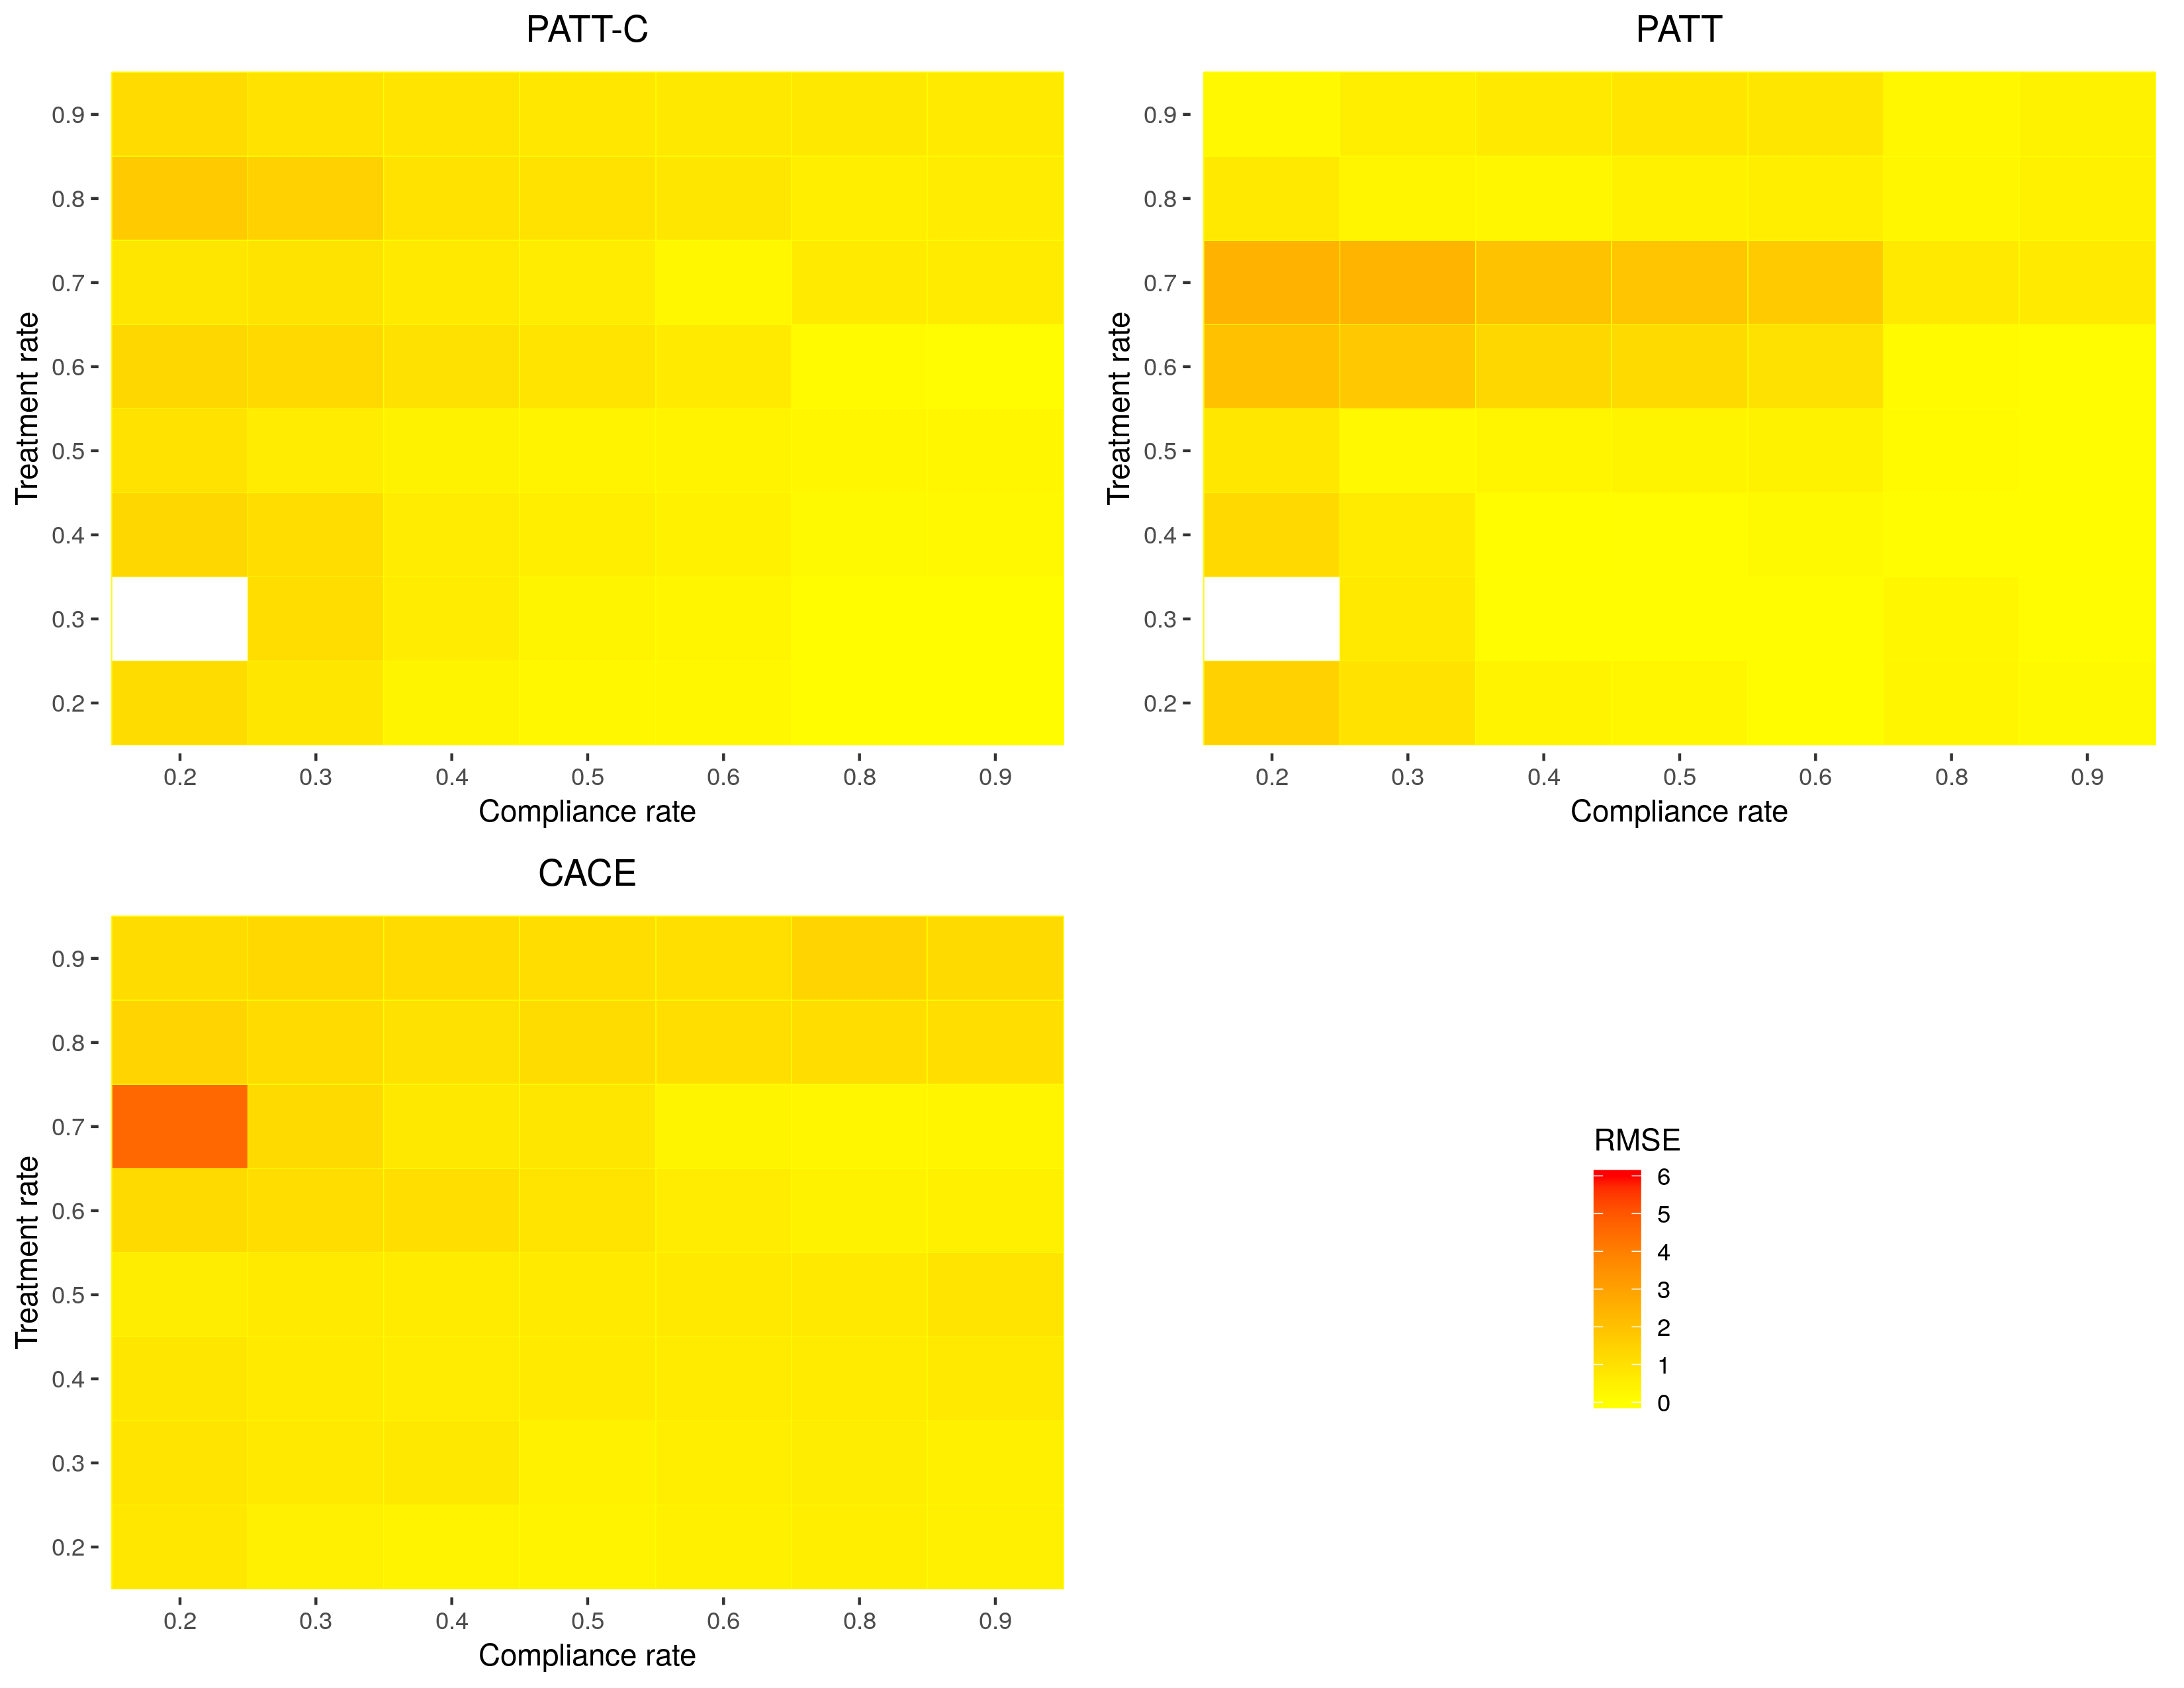
\includegraphics[width = 1\textwidth]{rmse_ratec_ratet.png}
		\caption{Simulated RMSE, binned by compliance rate and treatment rate. \label{fig:rmse_ratec_ratet}}
%		\caption{\label{fig:rmse_ratec_ratet} here}
	\end{center}
\end{figure}

\begin{figure}[htbp]
	\begin{center}
		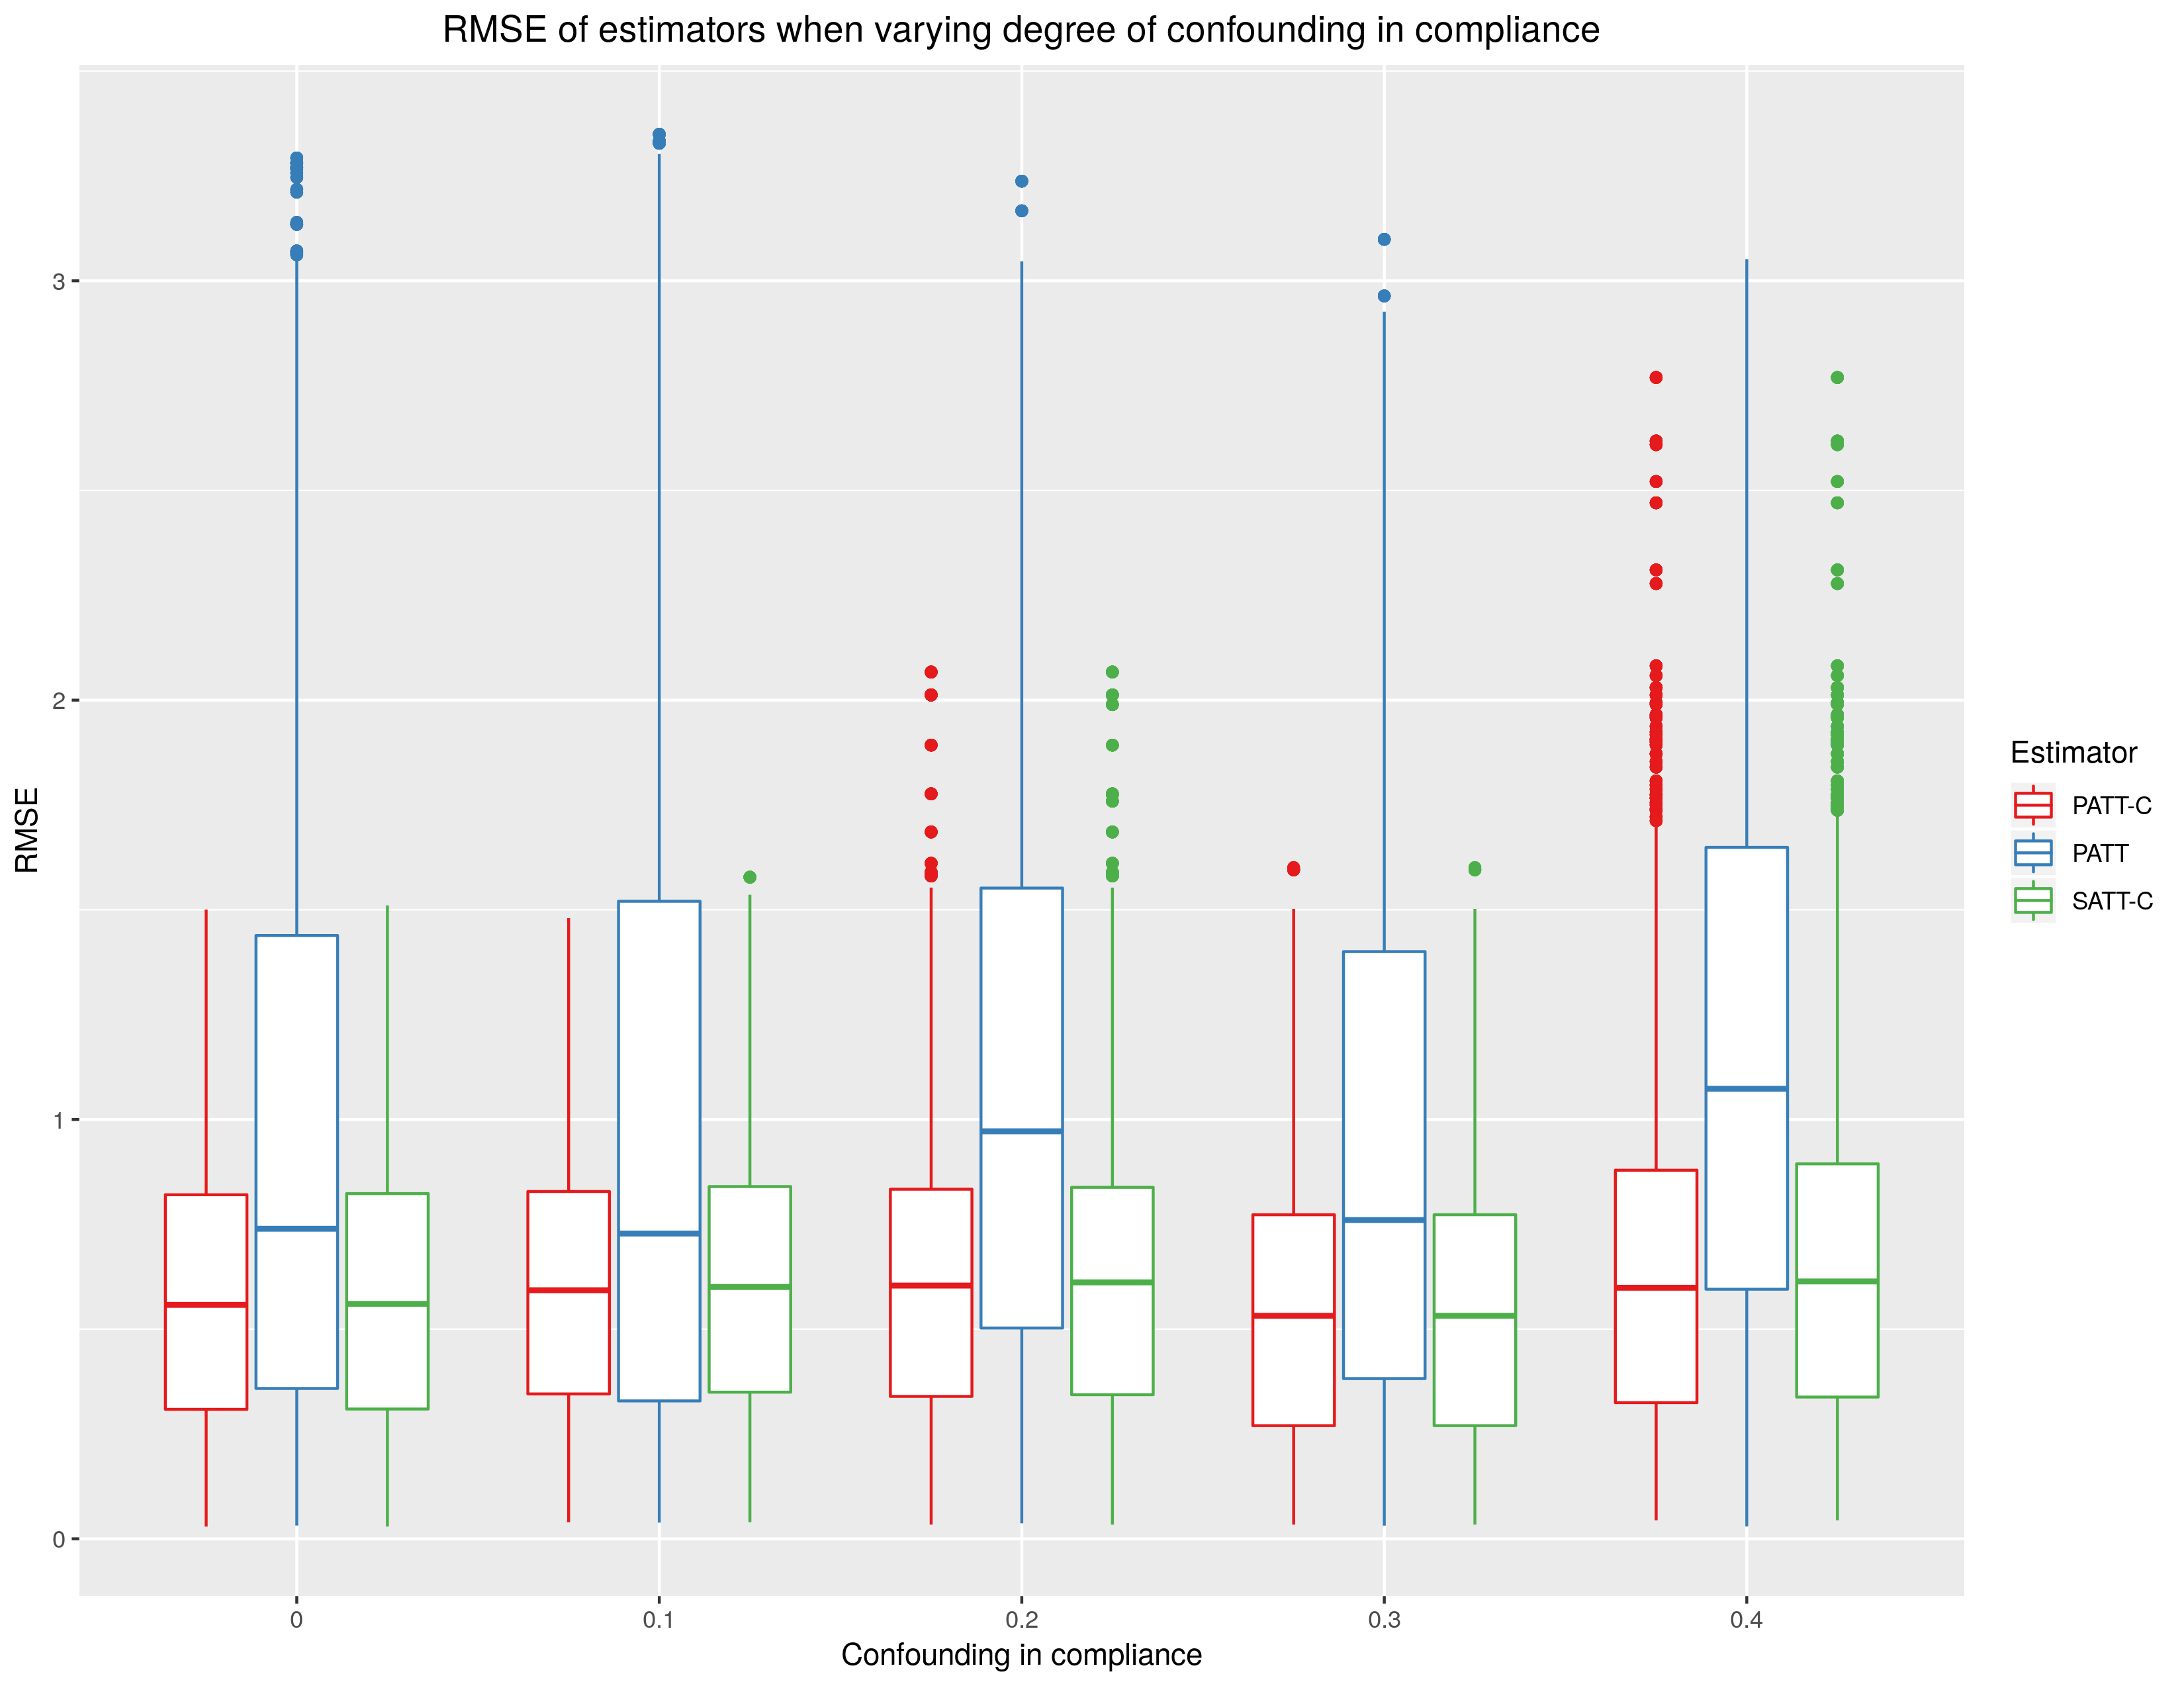
\includegraphics[width = 1\textwidth]{rmse_boxplots_RateConC.png}
		\caption{Simulated RMSE of PATT-C, PATT, and CACE, according to degree of confounding in compliance.\label{fig:rmse_boxplots_RateConC}}
	%	\caption{\label{fig:rmse_boxplots_RateConC} here}
	\end{center}
\end{figure}

\begin{figure}[htbp]
	\begin{center}
		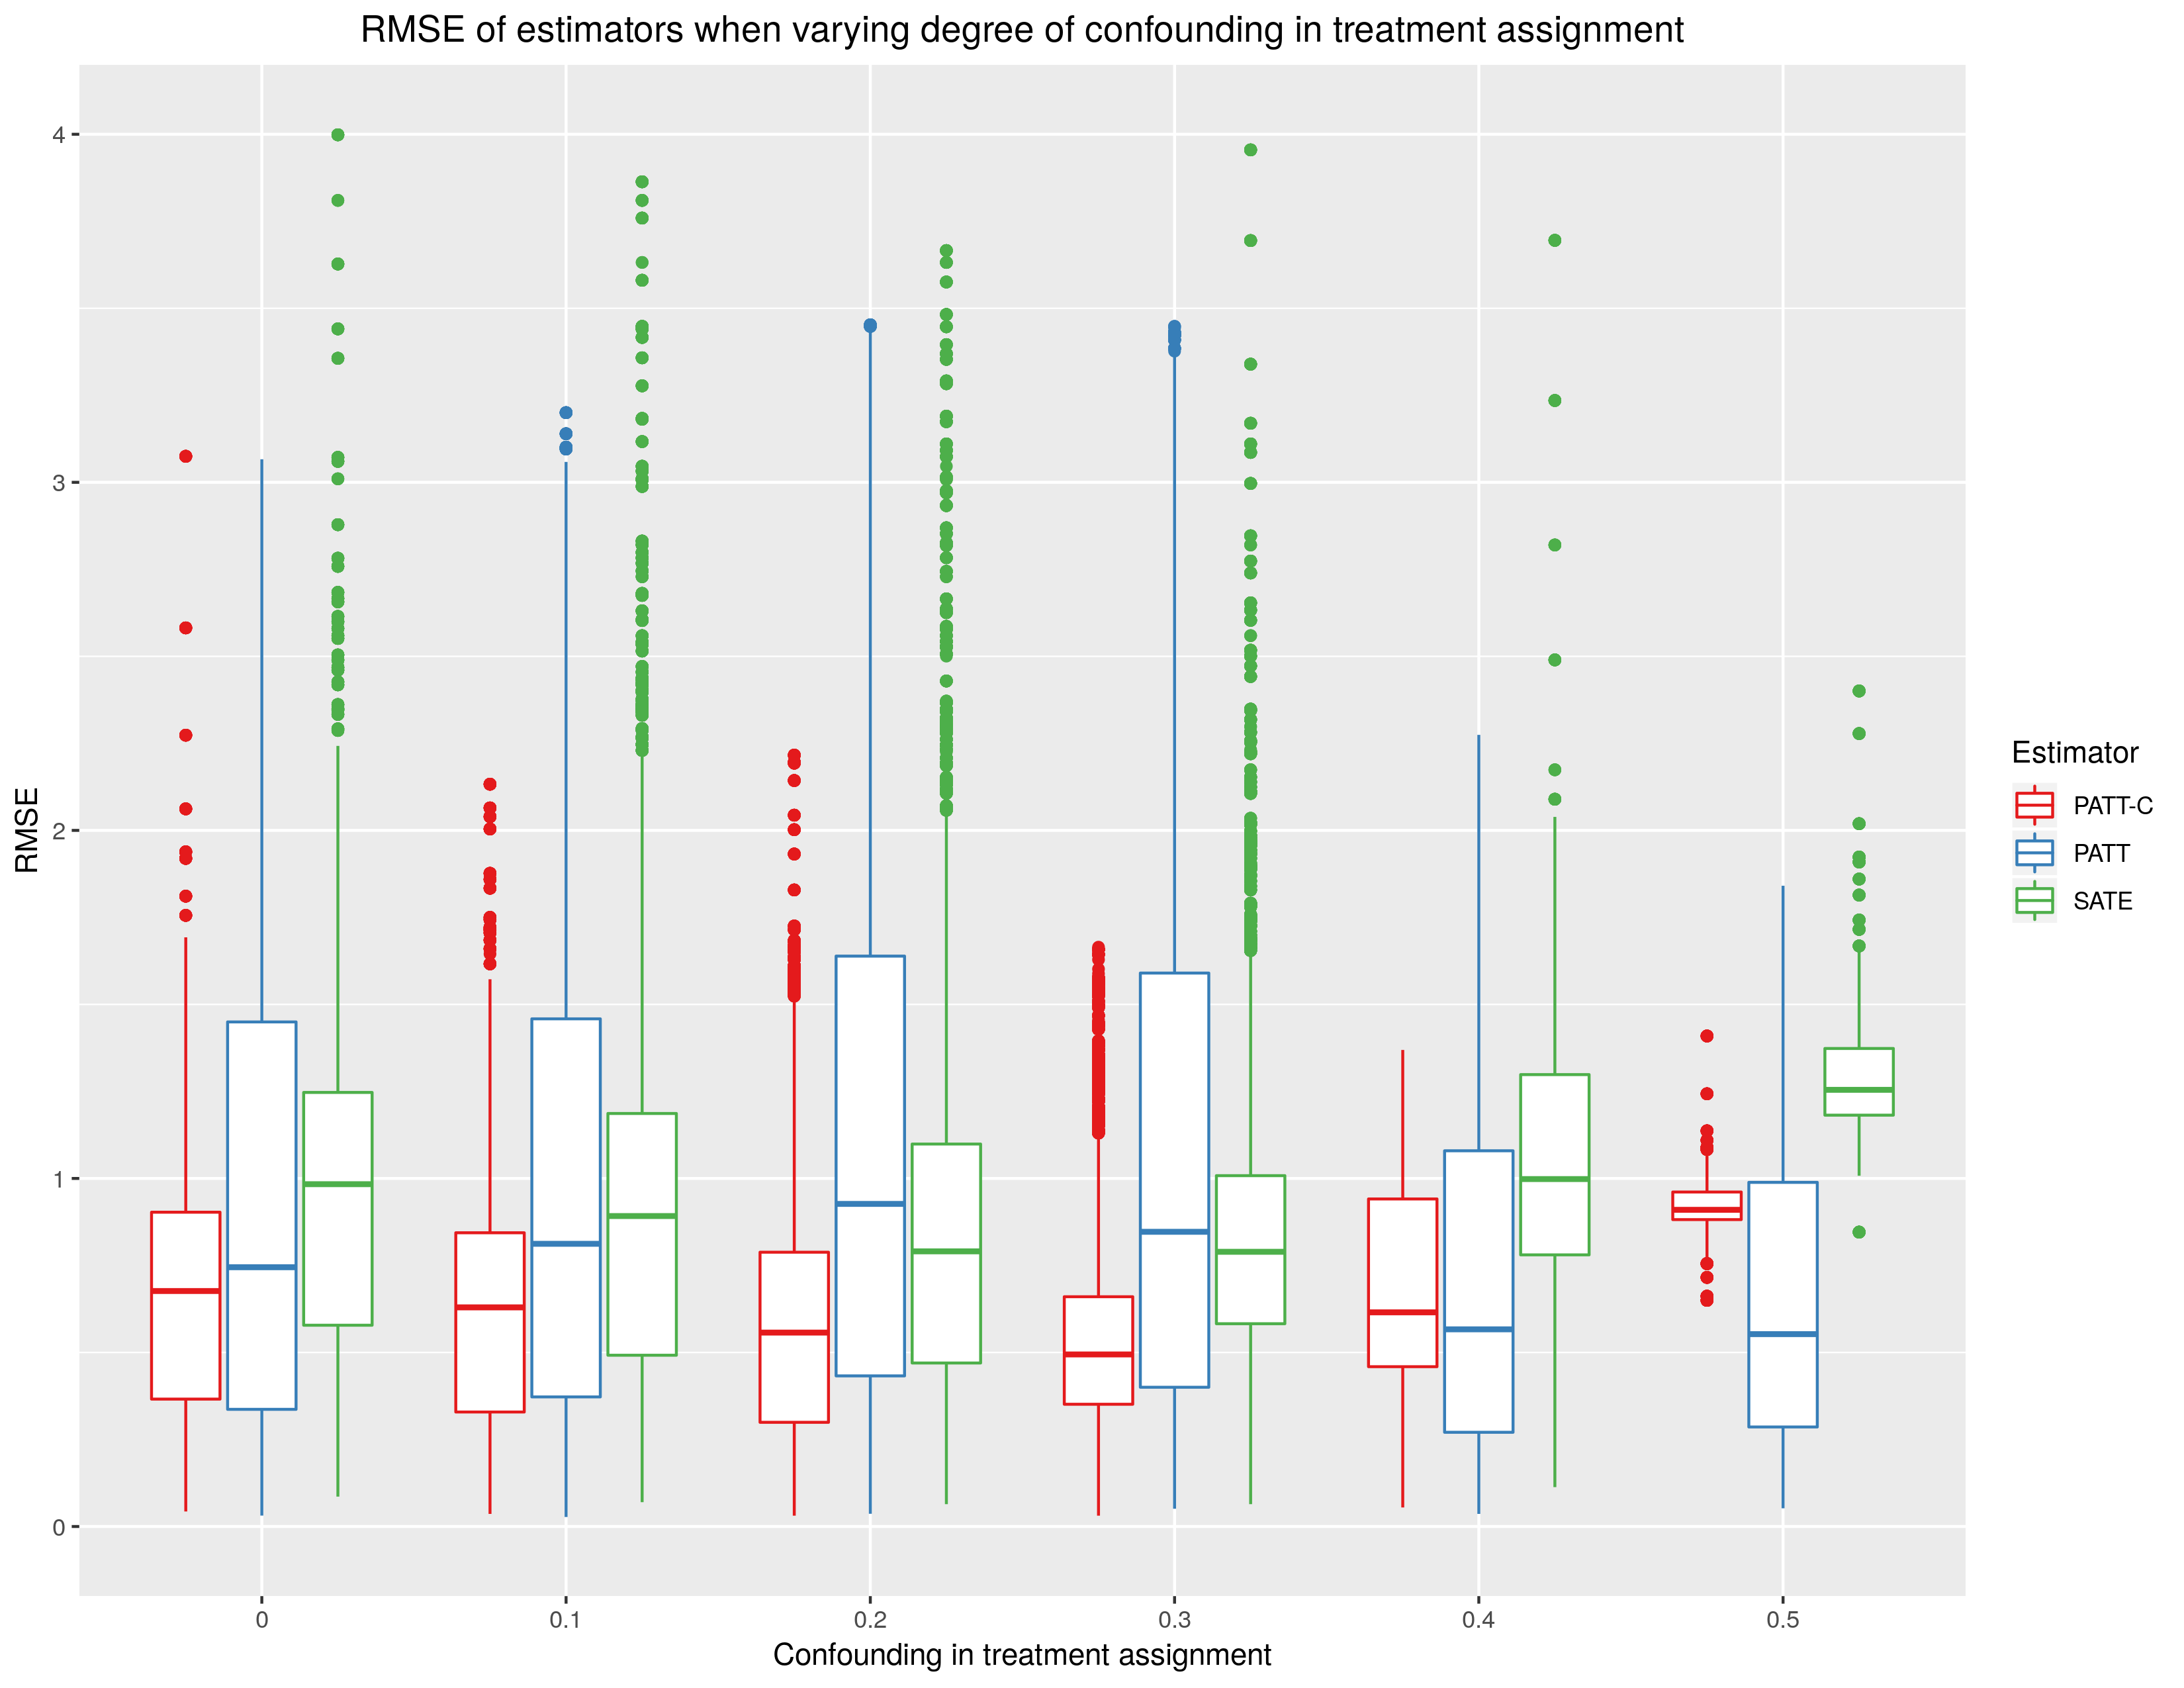
\includegraphics[width = 1\textwidth]{rmse_boxplots_RateConT.png}
		\caption{Simulated RMSE of PATT-C, PATT, and CACE, according to degree of confounding in treatment assignment.\label{fig:rmse_boxplots_RateConT}}
	%		\caption{\label{fig:rmse_boxplots_RateConT} here}
	\end{center}
\end{figure}

\begin{figure}[htbp]
	\begin{center}
		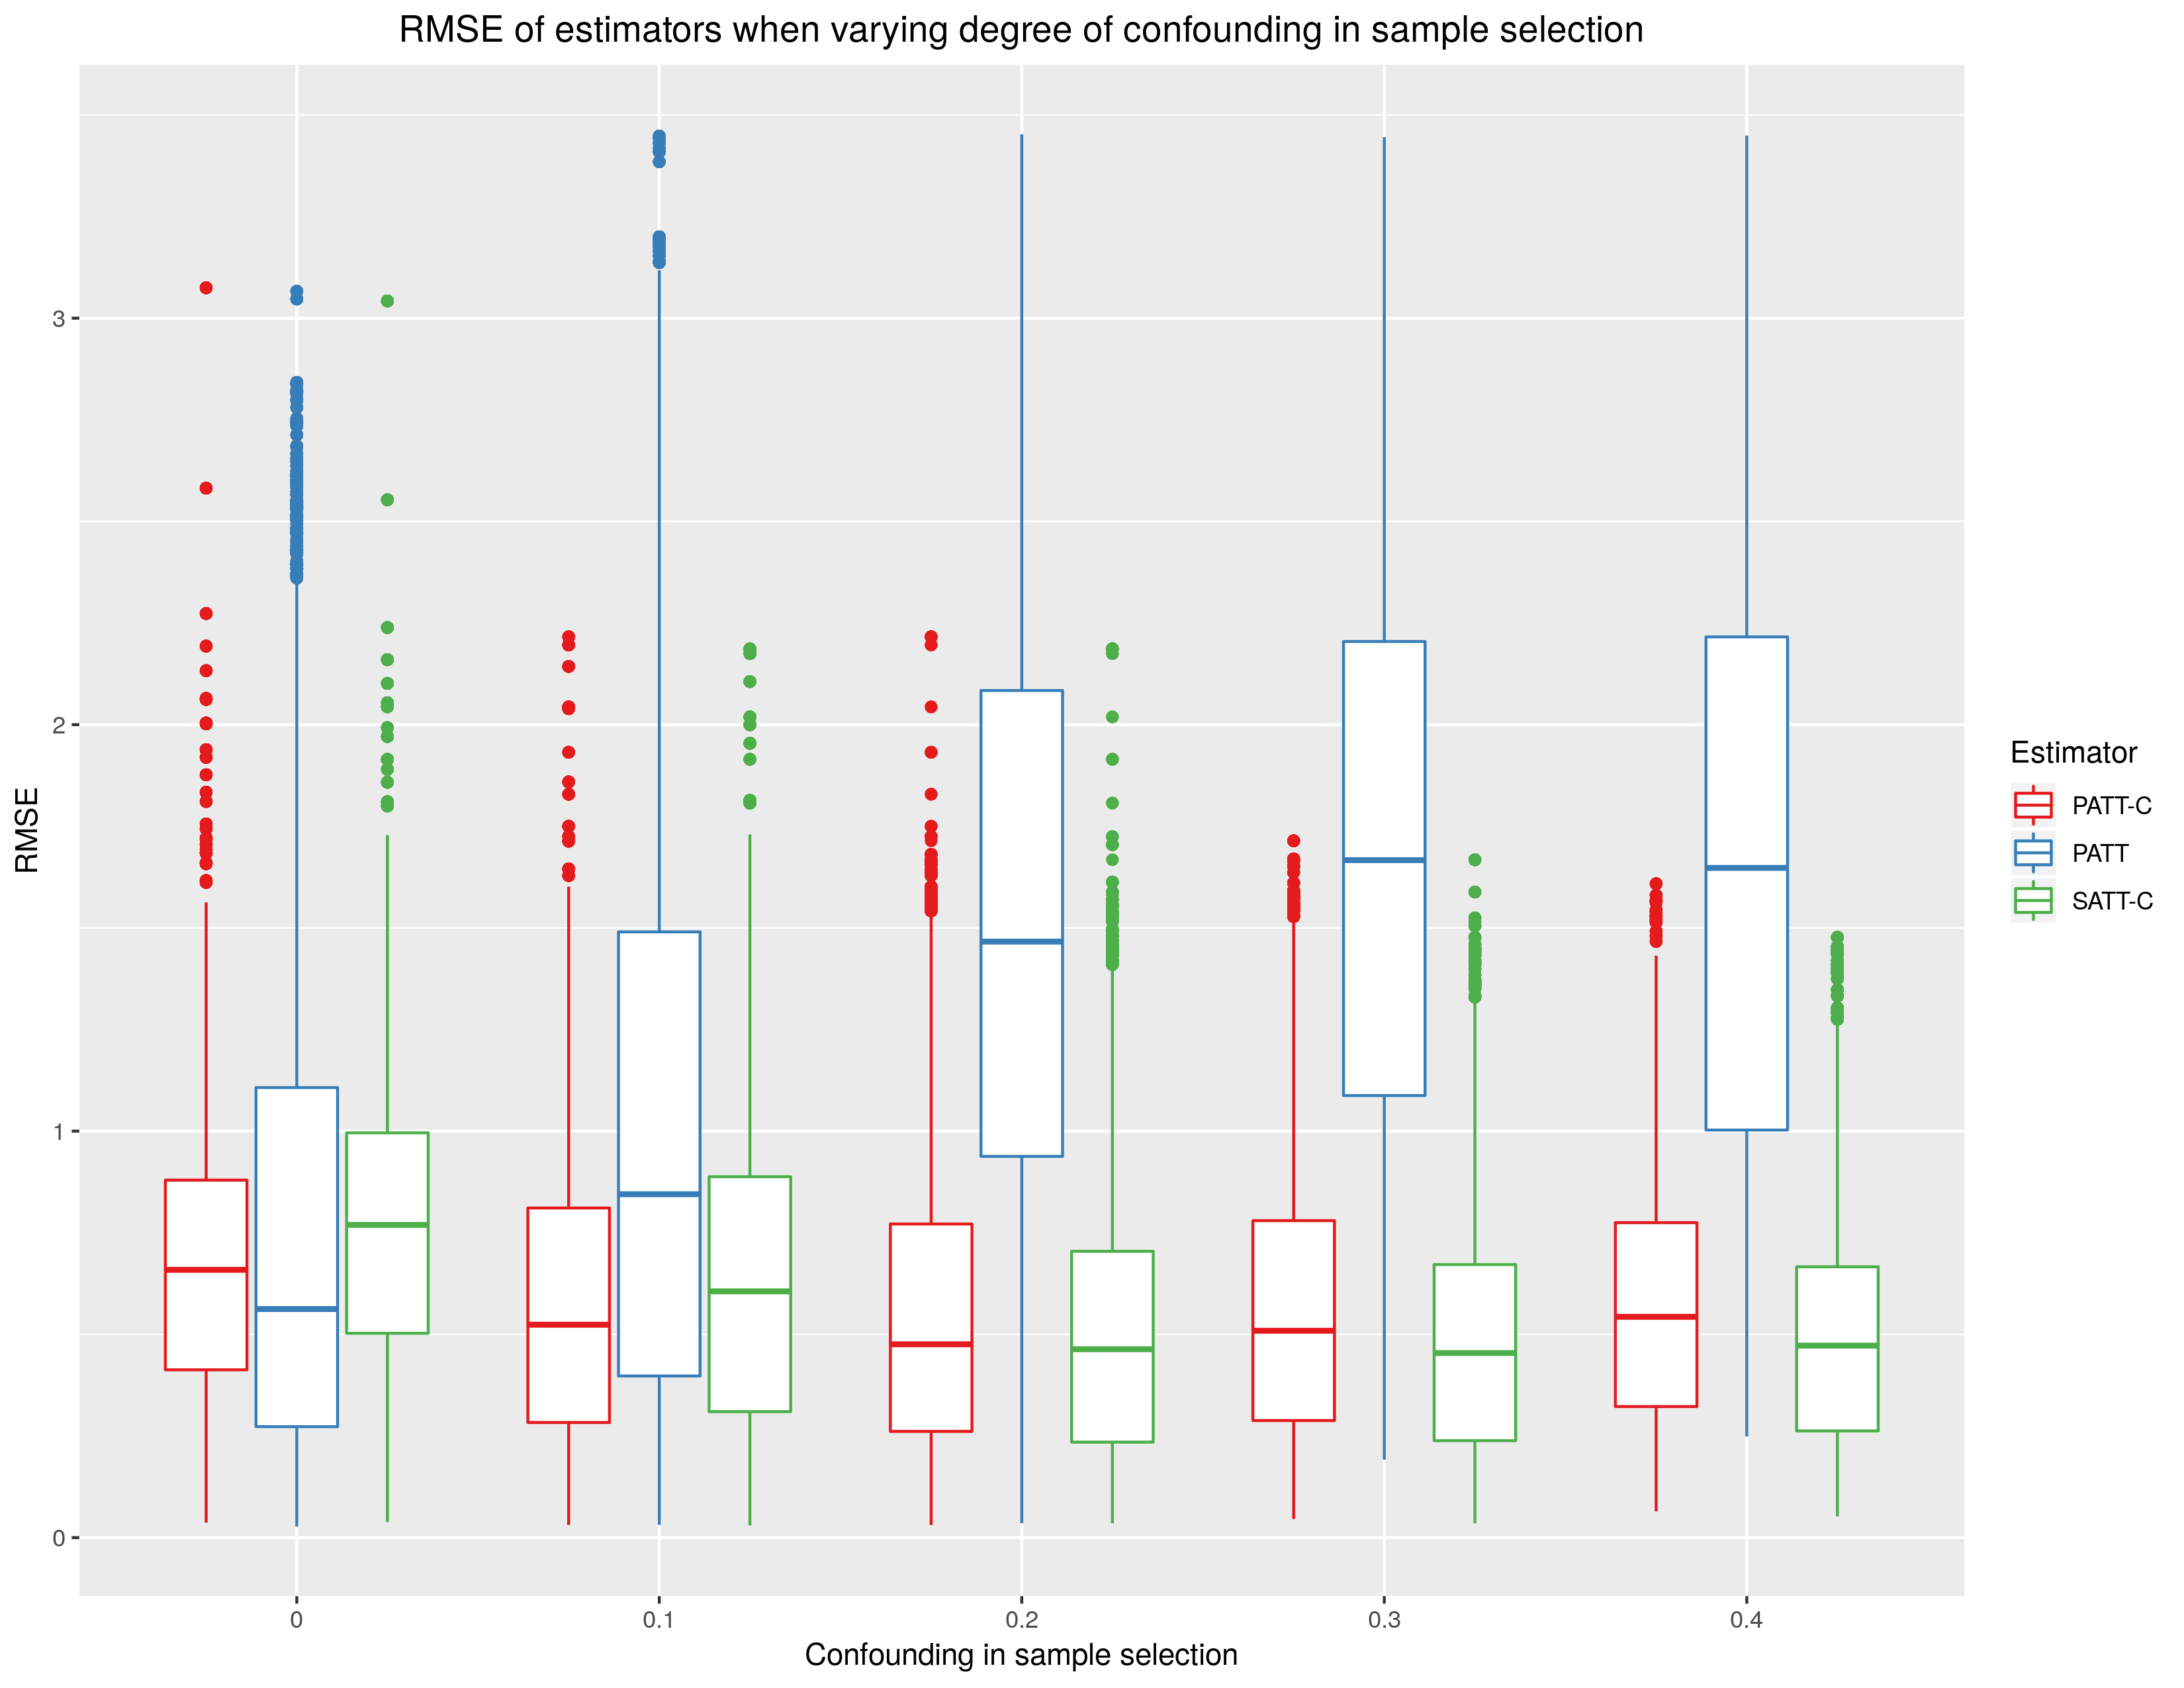
\includegraphics[width = 1\textwidth]{rmse_boxplots_RateConS.png}
		\caption{Simulated RMSE of PATT-C, PATT, and CACE, according to degree of confounding in sample selection.\label{fig:rmse_boxplots_RateConS}}
	%		\caption{\label{fig:rmse_boxplots_RateConS} here}
	\end{center}
\end{figure}

\newgeometry{left=3cm,bottom=0.1cm}
\begin{singlespace}
	\begin{longtable}{lllllll}
		\caption{Pretreatment covariates and responses for OHIE and NHIS respondents by Medicaid coverage status.\label{rct-nrt-compare}} \\
		& OHIE &  & OHIE &  & NHIS &  \\ 
		& no Medicaid &  & Medicaid &  &Medicaid &   \\ 
		& $n=4,519$ &  & $n=6,100$ &  & $n=6,261$ &  \\  
		\hline   
		\hline   
		\textbf{Covariate} &  $\mathbf{n}$ & $\mathbf{\%}$ & $\mathbf{n}$ & $\mathbf{\%}$ & $\mathbf{n}$ & $\mathbf{\%}$ \\ 
		\hline
		\textit{Sex:} &  & & &  &  & \\ 
		
		\hspace{3mm} Female & 2,538 & 56.2 & 3506 & 57.5 & 4,288 & 68.5 \\ 
		&  & & &  &  & \\ 
		\textit{Age:} &  & & &  &  & \\ 
		\hspace{3mm}19-49 & 1,288 & 28.5 & 1,625 & 26.6 & 4324 & 69.1  \\ 
		
		\hspace{3mm}50-64 & 3,231 & 71.5 & 4,475 & 73.4 & 1,937 & 30.9 \\ 
		&  & & &  &  & \\ 
		\textit{Race:} &  & & &  &  & \\ 
		\hspace{3mm}White & 3,956 & 87.5 & 5,183 & 85.0 & 3,902 & 62.3  \\ 
		
		\hspace{3mm}Black & 193 & 4.3 & 247 & 4.0 & 1,723 & 27.5  \\ 
		
		\hspace{3mm}Hispanic &  264 & 5.8 & 538 & 8.8 & 1,570 & 25.1  \\ 
		&  & & &  &  & \\ 
		\textit{Health status:} &  & & &  &  & \\ 
		\hspace{3mm}Diabetes & 459 & 10.2 & 637 & 10.4 & 866 & 13.8  \\ 
		
		\hspace{3mm}Asthma & 823 & 18.2 & 1,094 & 17.9 & 1272 & 20.3   \\ 
		
		\hspace{3mm}High blood pressure & 1,362 & 30.1 & 1,705 & 27.9 & 2,166 & 34.6  \\ 
		
		\hspace{3mm}Heart condition & 120 & 2.7 & 189 & 3.1 & 529 & 8.4 \\ 
		&  & & &  &  & \\ 
		\textit{Education:} &  & & &  &  & \\  
		\hspace{3mm}Less than high school  & 858 & 19.0 & 1,154 & 18.9 & 1,942 & 31.0  \\ 
		
		\hspace{3mm}High school diploma or GED & 2,589 & 57.3 & 3,279 & 53.8 & 2,076 & 33.2   \\ 
		
		\hspace{3mm}Voc. training / 2-year degree & 804 & 17.8 & 1,186 & 19.4 & 1,810 & 28.9  \\ 
		
		\hspace{3mm}4-year college degree or more & 268 & 5.9 & 481 & 7.9 & 433 & 6.9  \\ 
		&  & & &  &  & \\ 
		\textit{Income:} &  & & &  &  & \\ 
		\hspace{3mm} $<\$10$k & 4,518 & 100.0 & 4,111 & 67.4 & 2,588 & 41.3  \\
		
		\hspace{3mm} \$10k-\$25k & 1 & 0.0 & 1,616 & 26.5 & 3,098 & 49.5 \\
		
		\hspace{3mm} $>\$25$k & 0 & 0.0 & 373 & 6.1 & 575 & 9.2   \\
		\hline
		\hline
		\textbf{Binary response} &  $\mathbf{n}$ & $\mathbf{\%}$ & $\mathbf{n}$ & $\mathbf{\%}$ & $\mathbf{n}$ & $\mathbf{\%}$ \\ 
		\hspace{3mm}Any ER visit &  1,377 & 25.4 & 1,301 & 25.1 & 1,659 & 26.5  \\  
		%\hspace{3mm}Any outpatient visit & 3,265 & 60.2 & 3,081 & 59.3 & 4,093 & 65.4 \\
		\hline
		\textbf{Continuous response} &  $\mathbf{\bar{x}}$ & $\mathbf{sd}$& $\mathbf{\bar{x}}$ & $\mathbf{sd}$ & $\mathbf{\bar{x}}$ & $\mathbf{sd}$ \\  
		\hspace{3mm}$\#$ ER visits &  0.44 & 0.95 & 0.44 & 0.99 & 0.48 & 1.0  \\  
		\hspace{3mm}$\#$ outpatient visits & 1.9 & 3.01 & 1.9 & 2.8 & 2.08 & 2.3 \\
		\hline
		\hline
	\end{longtable}
\end{singlespace}
\restoregeometry

\begin{table}[h]
	\begin{center}
	\caption{Distribution of OHIE participants by status of treatment assignment ($T_i$) and treatment received ($D_i$).\label{ohie-status}} 
	\begin{tabular}{@{}lccc@{}}
		\toprule
		& $D_i = 0$ & $D_i = 1$ & n      \\ \midrule
		$T_i = 0$ & 10,010    & 1,556     & 11,566 \\
		$T_i = 1$ & 6,446     & 5,193     & 11,639 \\
		n         & 16,456    & 6,749     & 23,205 \\ \bottomrule
	\end{tabular}
	\end{center}
\end{table}

\begin{table}[h]
	\begin{center}
		\caption{Placebo test results comparing the mean outcomes of RCT compliers and adjusted population ``compliers.''\label{placebo}} 
	\begin{tabular}{@{}lcccc@{}}
		\toprule
		Outcome                & RCT complier & Adjusted pop. ``complier" & Difference & $p$-value \\
				                &  mean & mean & &  \\		
		 \midrule
		Any ER visit           & 0.25              & 0.25                           & 0.0001     & 0.97    \\
		$\#$ ER vists          & 0.45              & 0.45                           & 0.002      & 0.85    \\
		$\#$ outpatient visits & 1.90              & 1.94                           & -0.03      & 0.26    \\ \bottomrule
	\end{tabular}
\end{center}
\footnotesize{Notes: $p$-values for difference-in-means calculated from two-sided t-test.}
\end{table}

\begin{table}[h]
	\caption{Comparison of population and sample estimates.\label{compliance-compare}} 
	\begin{tabular}{@{}llll@{}}
		\toprule
		\backslashbox{Estimator}{Outcome} 				& Any ER visit 	& $\#$ ER visits   & $\#$ outpatient visits      \\ \midrule
		PATT-C                                           & 0.0001 [0.0001, 0.0001]   & 0.0005 [0.0002, 0.0008]	& 0.002 [0.002, 0.002] \\
		PATT                                             & 0.0006 [0.0005, 0.0007]   & -0.004 [-0.005, -0.004]	& 0.02 [0.02, 0.02]  \\
		CACE                                             & -0.001 [-0.02, 0.02]   & 0.005 [-0.05, 0.06]	& -0.02 [-0.19, 0.14]  \\ \bottomrule
	\end{tabular}\\
	\footnotesize{Notes: Estimates in brackets represent 95\% bootstrap confidence intervals constructed with 1,000 bootstrap samples.}
\end{table}

\begin{figure}[htbp]
	\begin{center}
		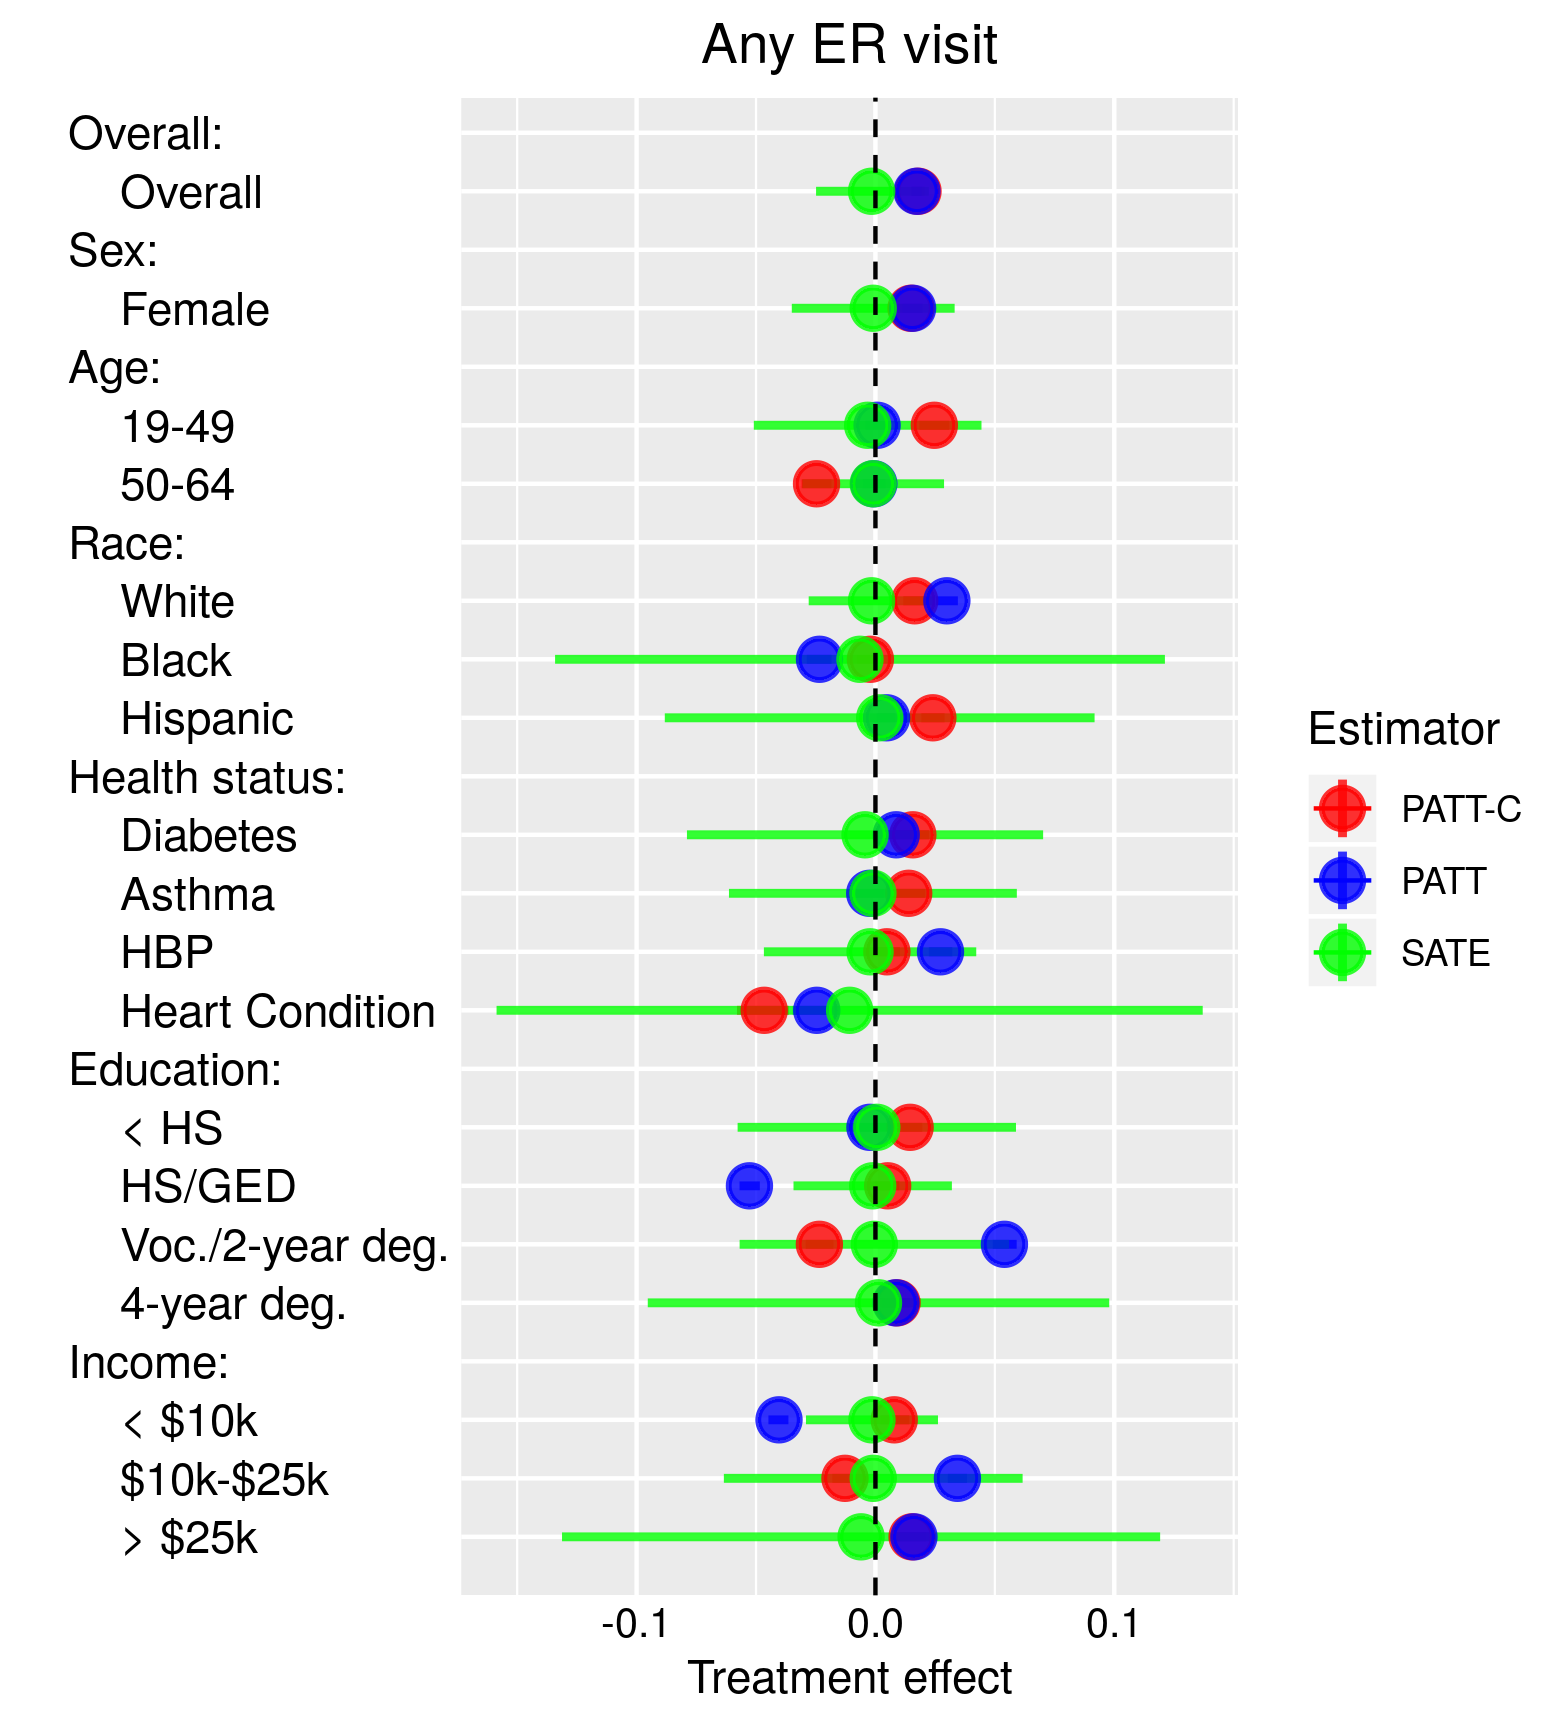
\includegraphics[width = 0.9\textwidth]{any-visit-plot.png}
		\caption{Heterogeneity in sample and population treatment effect estimates: any ER visit. Horizontal lines represent 95\% bootstrap confidence intervals constructed with 1,000 bootstrap samples.\label{fig:any-visit-plot}}
		%	\caption{\label{fig:any-visit-plot} here}
	\end{center}
\end{figure}


\begin{figure}[htbp]
	\begin{center}
		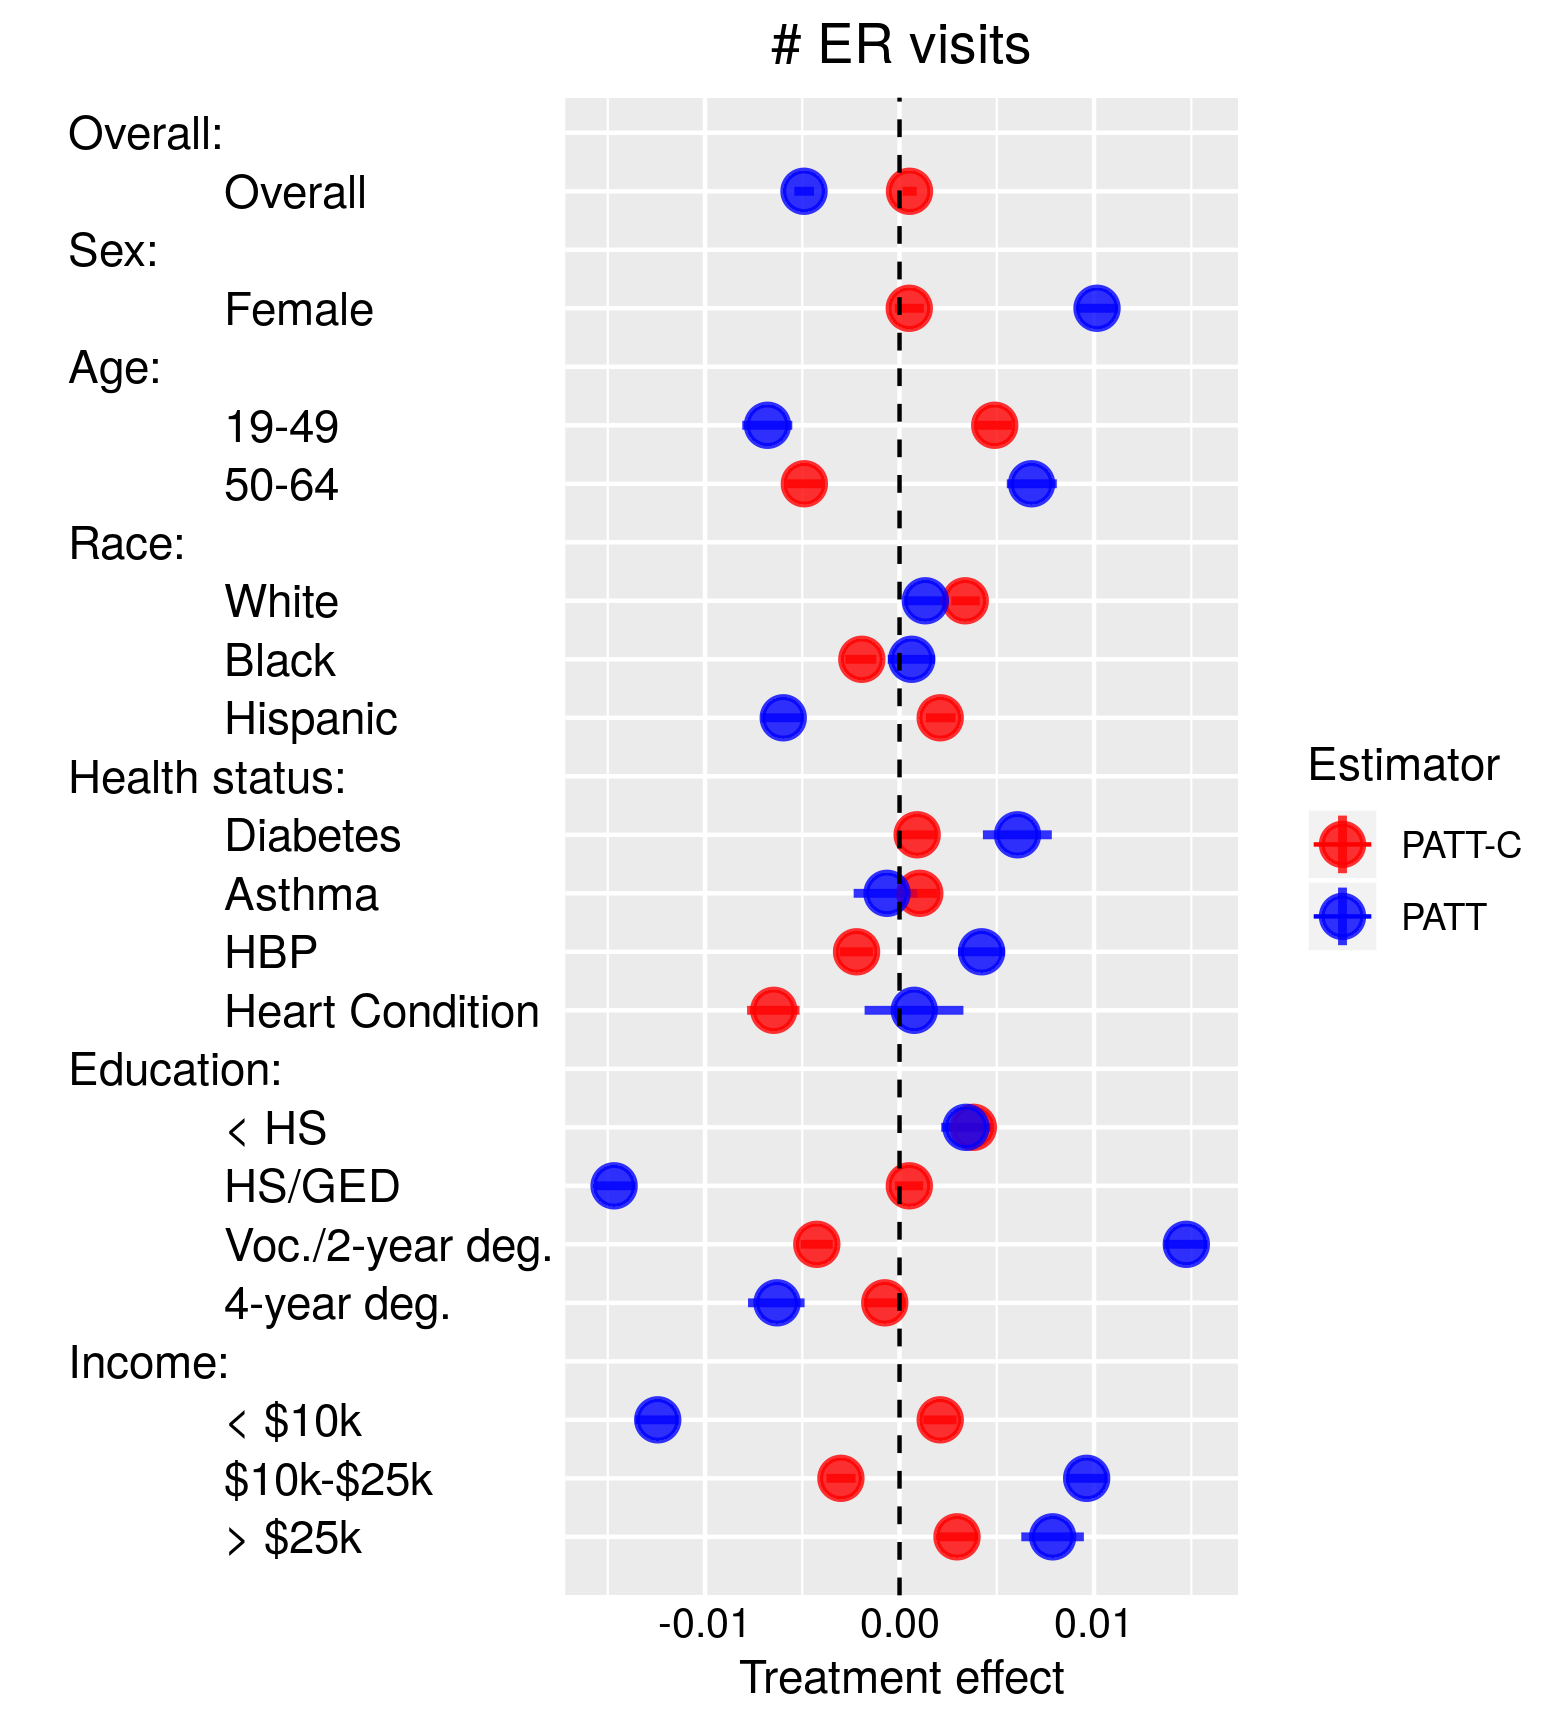
\includegraphics[width = 0.9\textwidth]{num-visit-plot.png}
		\caption{Heterogeneity in population treatment effect estimates: $\#$ ER visits.\label{fig:num-visit-plot}}
		%	\caption{\label{fig:num-visit-plot} here}
	\end{center}
\end{figure}

\begin{figure}[htbp]
	\begin{center}
		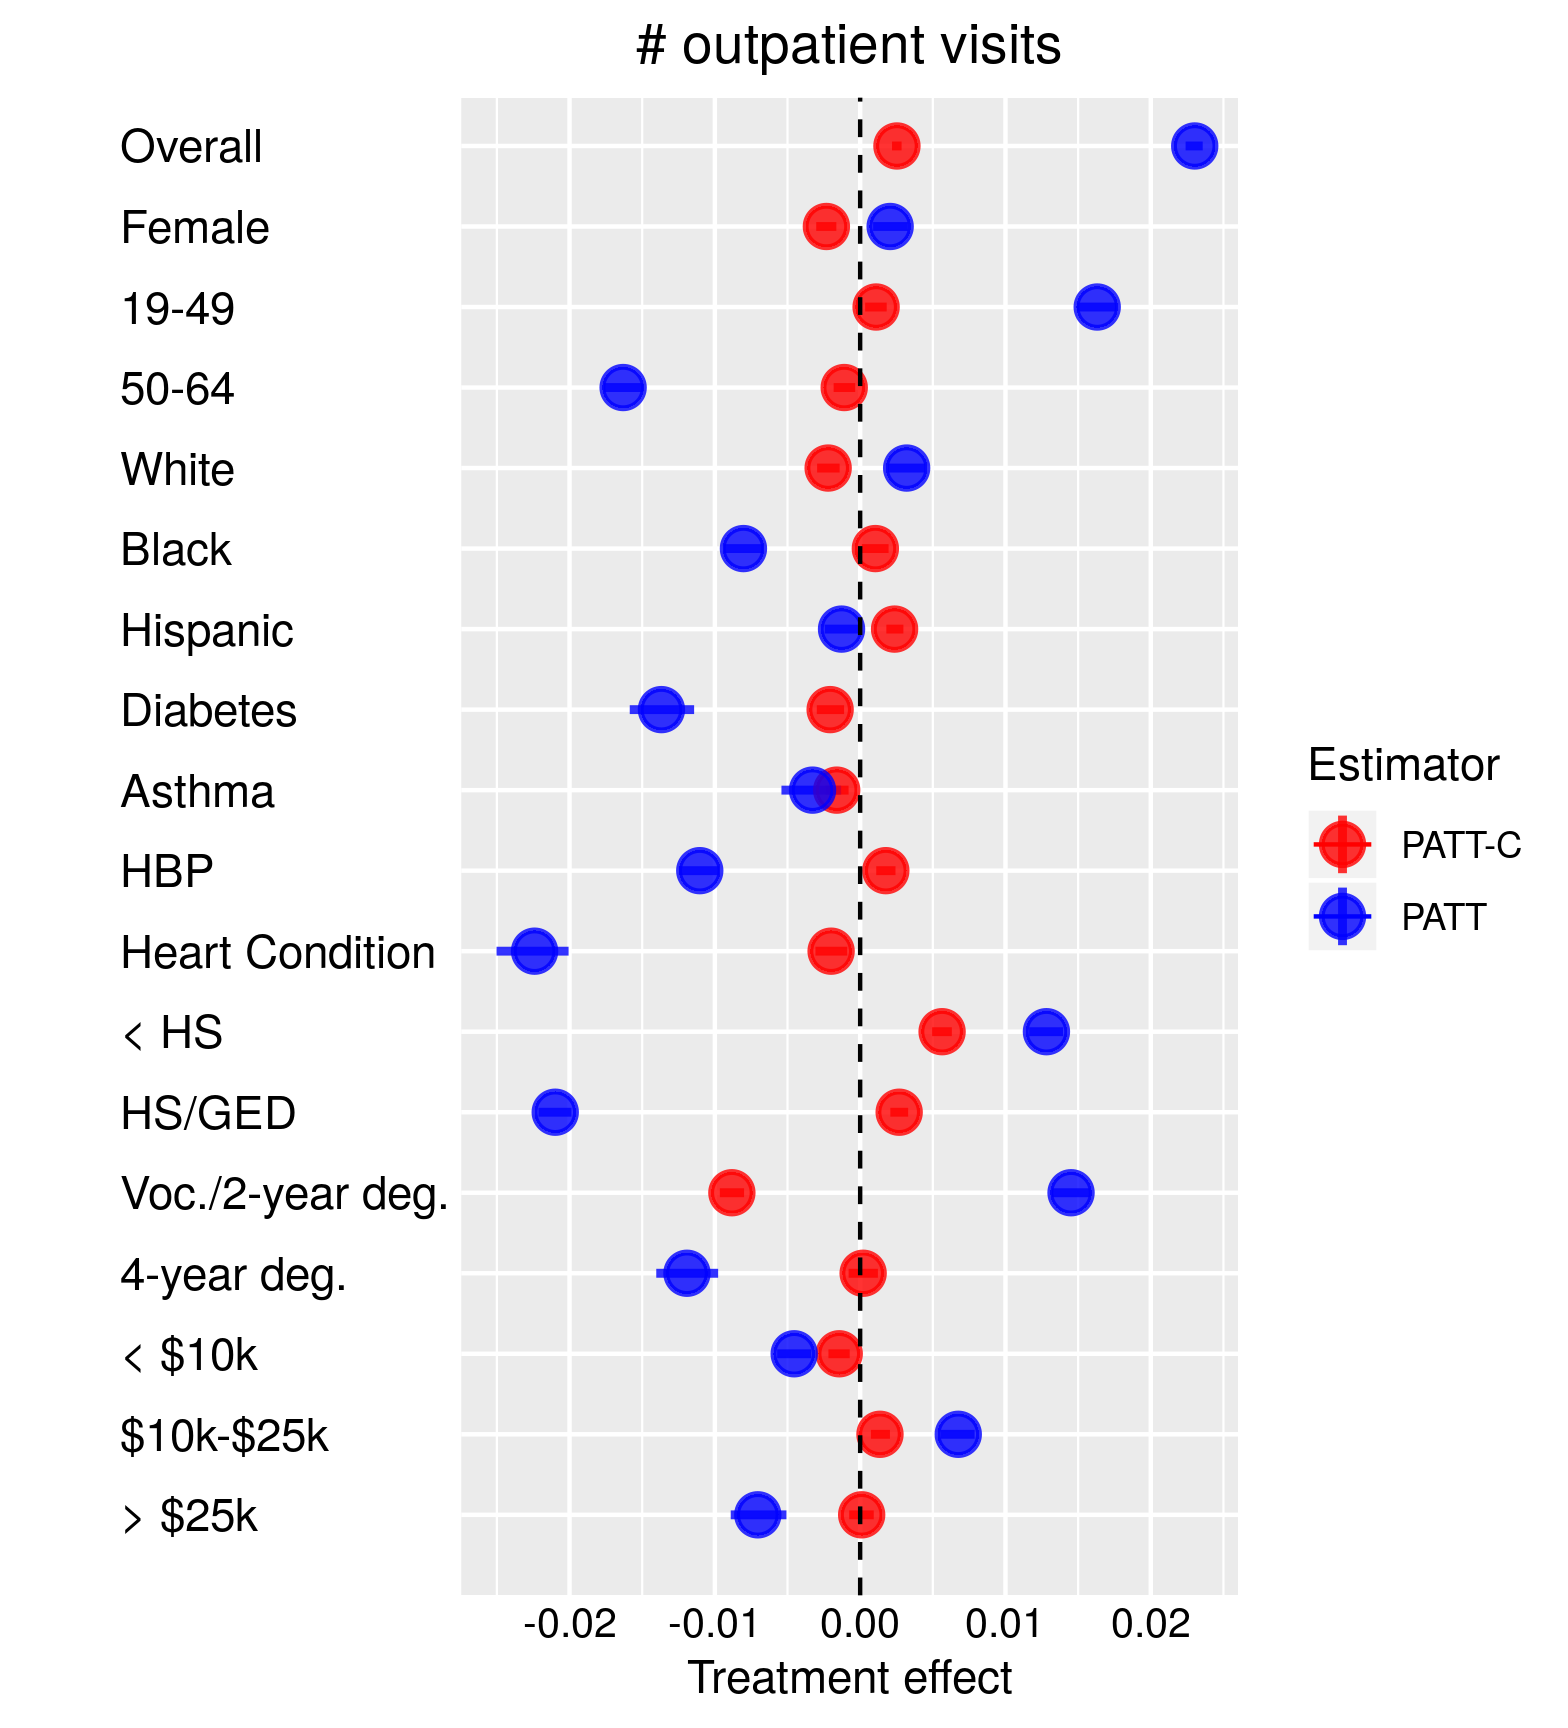
\includegraphics[width = 0.9\textwidth]{num-out-plot.png}
		\caption{Heterogeneity in population treatment effect estimates: $\#$ outpatient visits.\label{fig:num-out-plot}}
		%	\caption{\label{fig:num-out-plot} here}
	\end{center}
\end{figure}

% complier-mod
\begin{table}[h]
\begin{center}
\caption{Distribution of MSE for compliance ensemble.\label{compliance-ensemble}} 
\begin{tabular}{lcccc}
  \hline
 Algorithm & Mean & SE & Min. & Max. \\ 
  \hline
        \rowcolor{Gray}
Super learner (\texttt{SuperLearner}) & 0.22  & 0.001 & 0.21 & 0.23 \\
%Discrete SL & 0.22  & 0.001 & 0.21 & 0.23 \\
Lasso regression (\texttt{glmnet})  & 0.22  & 0.001 & 0.21 & 0.23 \\
Random forests (\texttt{randomForest}) & 0.27  & 0.002 & 0.25 & 0.29 \\
Ridge regression (\texttt{glmnet}) & 0.22  & 0.001 & 0.21 & 0.23 \\
   \hline
\end{tabular} 
\end{center}
\footnotesize{Notes: MSE is 10-fold cross-validated error for super learner ensemble and candidate algorithms. \textsf{R} package used for implementing each algorithm in parentheses.}
\end{table}

\pagebreak

\begin{table}[h]
\caption{Error and weights for candidate algorithms in response ensemble for RCT compliers.\label{reponse-ensemble}}  
  \begin{tabularx}{\linewidth}{l*{3}{Y}}
    \toprule
    \multicolumn{3}{l}{\textbf{Any ER visit}} \\
    \midrule
 Algorithm &  MSE & Weight \\ 
  \hline
Lasso regression (\texttt{glmnet})  & 0.18 & 1 \\ 
Random forests, $\# preds. = 1$ (\texttt{randomForest}) & 0.25 & 0 \\ 
Random forests, $\# preds. = 10$ (\texttt{randomForest}) & 0.24 & 0 \\ 
Regularized logistic regression, $\alpha=0.25$ (\texttt{glmnet})  & 0.19 & 0 \\ 
Regularized logistic regression, $\alpha=0.5$ (\texttt{glmnet})  & 0.19 & 0 \\ 
Regularized logistic regression, $\alpha=0.75$ (\texttt{glmnet})  & 0.19 & 0 \\ 
Ridge regression (\texttt{glmnet})  & 0.18 & 0 \\ 
   \hline
  \end{tabularx}
  \begin{tabularx}{\linewidth}{l*{3}{Y}}
    \toprule
    \multicolumn{3}{l}{\textbf{$\#$ ER visits}} \\
    \midrule
Algorithm  & MSE & Weight \\ 
\hline
Additive regression, $\text{degree} = 3$ (\texttt{gam})  & 0.95 & 0 \\ 
Additive regression, $\text{degree} = 4$ (\texttt{gam})  & 0.95 & 0 \\ 
Lasso regression (\texttt{glmnet})  & 0.95 & 0.92 \\ 
Random forests, $\# preds. = 1$ (\texttt{randomForest}) & 0.95 & 0 \\ 
Random forests, $\# preds. = 10$ (\texttt{randomForest}) & 0.99 & 0.08 \\ 
Regularized linear regression, $\alpha=0.25$ (\texttt{glmnet})  & 0.95 & 0 \\ 
Regularized linear regression, $\alpha=0.5$ (\texttt{glmnet})  & 0.95 & 0 \\ 
Regularized linear regression, $\alpha=0.75$ (\texttt{glmnet})  & 0.95 & 0 \\ 
Ridge regression (\texttt{glmnet})  & 0.18 & 0 \\ 
   \hline
    \bottomrule
  \end{tabularx}
  \begin{tabularx}{\linewidth}{l*{3}{Y}}
	\toprule
	\multicolumn{3}{l}{\textbf{$\#$ outpatient visits}} \\
	\midrule
	Algorithm  & MSE & Weight \\ 
	\hline
	Additive regression, $\text{degree} = 3$ (\texttt{gam})  & 8.40 & 0 \\ 
	Additive regression, $\text{degree} = 4$ (\texttt{gam})  & 8.40 & 0 \\ 
	Lasso regression (\texttt{glmnet})  & 8.38 & 0 \\ 
	Random forests, $\# preds. = 1$ (\texttt{randomForest}) & 8.38 & 0 \\ 
	Random forests, $\# preds. = 10$ (\texttt{randomForest}) & 8.79 & 0.08 \\ 
	Regularized linear regression, $\alpha=0.25$ (\texttt{glmnet})  & 8.38 & 0 \\ 
	Regularized linear regression, $\alpha=0.5$ (\texttt{glmnet})  & 8.38 & 0 \\ 
	Regularized linear regression, $\alpha=0.75$ (\texttt{glmnet})  & 8.38 & 0.92 \\ 
	Ridge regression (\texttt{glmnet})  & 8.38 & 0 \\ 
	\hline
	\bottomrule
\end{tabularx}
\footnotesize{Notes: cross-validated error and weights used for each algorithm in super learner ensemble. \textit{MSE} is the ten-fold cross-validated mean squared error for each algorithm. \textit{Weight} is the coefficient for the Super Learner, which is estimated using non-negative least squares based on the Lawson-Hanson algorithm. \textsf{R} package used for implementing each algorithm in parentheses. $\# preds.$ is the number of predictors randomly sampled as candidates in each decision tree in random forests algorithm. $\alpha$ is a parameter that mixes L1 and L2 norms. $\text{degree}$ is the smoothing term for smoothing splines.}
\end{table}

\pagebreak

\begin{table}[ht]
\caption{Error and weights for candidate algorithms in response ensemble for all RCT participants.\label{reponse-ensemble-unadj}}  
  \begin{tabularx}{\linewidth}{l*{3}{Y}}
	\toprule
	\multicolumn{3}{l}{\textbf{Any ER visit}} \\
	\midrule
	Algorithm &  MSE & Weight \\ 
	\hline
	Lasso regression (\texttt{glmnet})  & 0.18 & 0.96 \\ 
	Random forests, $\# preds. = 1$ (\texttt{randomForest}) & 0.25 & 0 \\ 
	Random forests, $\# preds. = 10$ (\texttt{randomForest}) & 0.24 & 0.04 \\ 
	Regularized logistic regression, $\alpha=0.25$ (\texttt{glmnet})  & 0.18 & 0 \\ 
	Regularized logistic regression, $\alpha=0.5$ (\texttt{glmnet})  & 0.18 & 0 \\ 
	Regularized logistic regression, $\alpha=0.75$ (\texttt{glmnet})  & 0.18 & 0 \\ 
	\hline
\end{tabularx}
\begin{tabularx}{\linewidth}{l*{3}{Y}}
	\toprule
	\multicolumn{3}{l}{\textbf{$\#$ ER visits}} \\
	\midrule
	Algorithm  & MSE & Weight \\ 
	\hline
	Additive regression, $\text{degree} = 3$ (\texttt{gam})  & 0.94 & 0 \\ 
	Additive regression, $\text{degree} = 4$ (\texttt{gam})  & 0.94 & 0 \\ 
	Lasso regression (\texttt{glmnet})  & 0.93 & 0.88 \\ 
	Random forests, $\# preds. = 1$ (\texttt{randomForest}) & 0.93 & 0 \\ 
	Random forests, $\# preds. = 10$ (\texttt{randomForest}) & 0.97 & 0.11 \\ 
	Regularized linear regression, $\alpha=0.25$ (\texttt{glmnet})  & 0.93 & 0 \\ 
	Regularized linear regression, $\alpha=0.5$ (\texttt{glmnet})  & 0.93 & 0 \\ 
	Regularized linear regression, $\alpha=0.75$ (\texttt{glmnet})  & 0.93 & 0 \\ 
	Ridge regression (\texttt{glmnet})  & 0.93 & 0 \\ 
	\hline
	\bottomrule
\end{tabularx}
\begin{tabularx}{\linewidth}{l*{3}{Y}}
	\toprule
	\multicolumn{3}{l}{\textbf{$\#$ outpatient visits}} \\
	\midrule
	Algorithm  & MSE & Weight \\ 
	\hline
	Additive regression, $\text{degree} = 3$ (\texttt{gam})  & 8.42 & 0 \\ 
	Additive regression, $\text{degree} = 4$ (\texttt{gam})  & 8.42 & 0 \\ 
	Lasso regression (\texttt{glmnet})  & 8.41 & 0 \\ 
	Random forests, $\# preds. = 1$ (\texttt{randomForest}) & 8.41 & 0.99 \\ 
	Random forests, $\# preds. = 10$ (\texttt{randomForest}) & 8.79 & 0.01 \\ 
	Regularized linear regression, $\alpha=0.25$ (\texttt{glmnet})  & 8.41 & 0 \\ 
	Regularized linear regression, $\alpha=0.5$ (\texttt{glmnet})  & 8.41 & 0 \\ 
	Regularized linear regression, $\alpha=0.75$ (\texttt{glmnet})  & 8.41 & 0 \\ 
	Ridge regression (\texttt{glmnet})  & 8.41 & 0 \\ 
	\hline
	\bottomrule
\end{tabularx}
\footnotesize{See notes to Fig.\ref{reponse-ensemble}.}
\end{table}

\end{appendices}

\itemize
\end{document}


